%
% 6.006 problem set 0 solutions template
%
\documentclass[11pt,twoside]{article}

\newcommand{\name}{}

\usepackage{amssymb}
\usepackage{amsmath}
\usepackage{graphicx}
\usepackage{latexsym}
\usepackage{times,url}
\usepackage{cprotect}
\usepackage{listings}
\usepackage{graphicx}
\usepackage[table]{xcolor}
\usepackage[letterpaper]{geometry}
\usepackage{tikz-qtree}
\usepackage{enumerate}

\newcommand{\profs}{Instructors: Dr. Nadi}
\newcommand{\subj}{6.006}
\newcommand{\ttt}[1]{{\tt\small #1}}

\definecolor{dkgreen}{rgb}{0,0.6,0}
\definecolor{dkblue}{rgb}{.2,.2,1}
\definecolor{gray}{rgb}{0.5,0.5,0.5}
\definecolor{mauve}{rgb}{0.58,0,0.82}

\lstset{
  language=Python,
  aboveskip=1pc,
  belowskip=1pc,
  basicstyle={\footnotesize\ttfamily},
  numbers=left,
  showstringspaces=false,
  numberstyle={\tiny\color{gray}\ttfamily},
  keywordstyle={\color{dkblue}\ttfamily},
  commentstyle={\color{dkgreen}\ttfamily},
  stringstyle={\color{mauve}\ttfamily},
}

% \lstset{
%   language=Python,
%   aboveskip=1pc,
%   belowskip=1pc,
%   basicstyle={\bf\color{white}\ttfamily},
%   numbers=left,
%   showstringspaces=false,
%   numberstyle={\bf\small\color{lightgray}\ttfamily},
%   keywordstyle={\bf\color{cyan}\ttfamily},
%   commentstyle={\bf\color{green}\ttfamily},
%   stringstyle={\bf\color{mauve}\ttfamily},
% }

\tikzset{
  % every node/.style={minimum width=2em,draw,circle},
  % level 1/.style={sibling distance=2cm},
  level distance=1cm,
  edge from parent/.style=
  {draw,edge from parent path={(\tikzparentnode) -- (\tikzchildnode)}},
}
\usetikzlibrary{shapes}

\newif\ifHideSolutions
\newcommand{\solutionBL}[1]{\textbf{Solution: }#1\color{black}}

\newif\ifHideSolutions
\newcommand{\solution}[1]{\color{dkgreen}\textbf{Solution: }#1\color{black}}
\newcommand{\commonmistakes}[1]{{\color{dkblue}\textbf{Common Mistakes: }#1}}
\newcommand{\rubric}[1]{\color{dkgreen}{\bf Rubric:} #1\color{black}}

% \HideSolutionsfalse
% \ifHideSolutions
%   \renewcommand{\solution}[1]{}
%   \renewcommand{\rubric}[1]{}
% \fi

\newlength{\toppush}
\setlength{\toppush}{2\headheight}
\addtolength{\toppush}{\headsep}

\newcommand{\htitle}[2]{\noindent\vspace*{-\toppush}\newline\parbox{0.5 \textwidth}
{\textit{Experiential Learning}\hfill   \name\newline
University of Tehran \hfill\newline
\profs 
\\[-3.5ex]\newline
}
\begin{minipage}{0.5\textwidth}
  \raggedleft % Equivalent to \flushright but often used in minipage for clarity
    \vspace{-0.37cm}
\includegraphics[width=1.75cm]{fig/Tehran-Uni-logo.png}\hspace*{0.22cm}
\end{minipage}
\mbox{}\hrulefill\mbox{}
\mbox{}\newline
\begin{center}{\Large\bf #1}\end{center}}

\newcommand{\handout}[2]{\thispagestyle{empty}
 \markboth{#1}{#1}
 \pagestyle{myheadings}\htitle{#1}{#2}}

\newcommand{\lecture}[3]{\thispagestyle{empty}
 \markboth{Lecture #1: #2}{Lecture #1: #2}
 \pagestyle{myheadings}\htitle{Lecture #1: #2}{#3}}

\newcommand{\htitlewithouttitle}[2]{\noindent\vspace*{-\toppush}\newline\parbox{6.5in}
{\textit{Introduction to Algorithms}\hfill#2\newline
Massachusetts Institute of Technology \hfill 6.006\newline
\profs\hfill Handout #1\vspace*{-.5ex}\newline
\mbox{}\hrulefill\mbox{}}\vspace*{1ex}\mbox{}\newline}

\newcommand{\handoutwithouttitle}[2]{\thispagestyle{empty}
 \markboth{Handout \protect\ref{#1}}{Handout \protect\ref{#1}}
 \pagestyle{myheadings}\htitlewithouttitle{\protect\ref{#1}}{#2}}

\newcommand{\exam}[2]{% parameters: exam name, date
 \thispagestyle{empty}
 \markboth{\hspace{1cm}\subj\ #1\hspace{1in}Name\hrulefill\ \ }%
          {\subj\ #1\hspace{1in}Name\hrulefill\ \ }
 \pagestyle{myheadings}\examtitle{#1}{#2}
 \renewcommand{\theproblem}{Problem \arabic{problemnum}}
}
\newcommand{\examsolutions}[3]{% parameters: handout, exam name, date
 \thispagestyle{empty}
 \markboth{Handout \protect\ref{#1}: #2}{Handout \protect\ref{#1}: #2}
% \pagestyle{myheadings}\htitle{\protect\ref{#1}}{#2}{#3}
 \pagestyle{myheadings}\examsolutionstitle{\protect\ref{#1}} {#2}{#3}
 \renewcommand{\theproblem}{Problem \arabic{problemnum}}
}
\newcommand{\examsolutionstitle}[3]{\noindent\vspace*{-\toppush}\newline\parbox{6.5in}
{\textit{Introduction to Algorithms}\hfill#3\newline
Massachusetts Institute of Technology \hfill 6.006\newline
%Singapore-MIT Alliance \hfill SMA5503\newline
\profs\hfill Handout #1\vspace*{-.5ex}\newline
\mbox{}\hrulefill\mbox{}}\vspace*{1ex}\mbox{}\newline
\begin{center}{\Large\bf #2}\end{center}}

\newcommand{\takehomeexam}[2]{% parameters: exam name, date
 \thispagestyle{empty}
 \markboth{\subj\ #1\hfill}{\subj\ #1\hfill}
 \pagestyle{myheadings}\examtitle{#1}{#2}
 \renewcommand{\theproblem}{Problem \arabic{problemnum}}
}

\makeatletter
\newcommand{\exambooklet}[2]{% parameters: exam name, date
 \thispagestyle{empty}
 \markboth{\subj\ #1}{\subj\ #1}
 \pagestyle{myheadings}\examtitle{#1}{#2}
 \renewcommand{\theproblem}{Problem \arabic{problemnum}}
 \renewcommand{\problem}{\newpage
 \item \let\@currentlabel=\theproblem
 \markboth{\subj\ #1, \theproblem}{\subj\ #1, \theproblem}}
}
\makeatother


\newcommand{\examtitle}[2]{\noindent\vspace*{-\toppush}\newline\parbox{6.5in}
{\textit{Introduction to Algorithms}\hfill#2\newline
Massachusetts Institute of Technology \hfill 6.006 Spring 2020\newline
%Singapore-MIT Alliance \hfill SMA5503\newline
\profs\hfill #1\vspace*{-.5ex}\newline
\mbox{}\hrulefill\mbox{}}\vspace*{1ex}\mbox{}\newline
\begin{center}{\Large\bf #1}\end{center}}

\newcommand{\grader}[1]{\hspace{1cm}\textsf{\textbf{#1}}\hspace{1cm}}

\newcommand{\points}[1]{[#1 points]\ }
\newcommand{\parts}[1]
{
  \ifnum#1=1
  (1 part)
  \else
  (#1 parts)
  \fi
  \ 
}

\newcommand{\bparts}{\begin{problemparts}}
\newcommand{\eparts}{\end{problemparts}}
\newcommand{\ppart}{\problempart}

%\newcommand{\lg} {lg\ }

\setlength{\oddsidemargin}{0pt}
\setlength{\evensidemargin}{0pt}
\setlength{\textwidth}{6.5in}
\setlength{\topmargin}{0in}
\setlength{\textheight}{8.5in}


\newcommand{\Spawn}{{\bf spawn} }
\newcommand{\Sync}{{\bf sync}}

\newcommand{\cif}[1]{\mbox{if $#1$}}
\newcommand{\cwhen}[1]{\mbox{when $#1$}}

\newcounter{problemnum}
\newcommand{\theproblem}{Problem \arabic{problemnum}}
\newenvironment{problems}{
        \begin{list}{{\bf \theproblem. \hspace*{0.5em}}}
        {\setlength{\leftmargin}{0em}
         \setlength{\rightmargin}{0em}
         \setlength{\labelwidth}{0em}
         \setlength{\labelsep}{0em}
         \usecounter{problemnum}}}{\end{list}}
\makeatletter
\newcommand{\problem}[1][{}]{\item \let\@currentlabel=\theproblem \textbf{#1}}
\makeatother

\newcounter{problempartnum}[problemnum]
\newenvironment{problemparts}{
        \begin{list}{{\bf (\alph{problempartnum})}}
        {\setlength{\leftmargin}{2.5em}
         \setlength{\rightmargin}{2.5em}
         \setlength{\labelsep}{0.5em}}}{\end{list}}
\newcommand{\problempart}{\addtocounter{problempartnum}{1}\item}

\newenvironment{truefalseproblemparts}{
        \begin{list}{{\bf (\alph{problempartnum})\ \ \ T\ \ F\hfil}}
        {\setlength{\leftmargin}{4.5em}
         \setlength{\rightmargin}{2.5em}
         \setlength{\labelsep}{0.5em}
         \setlength{\labelwidth}{4.5em}}}{\end{list}}

\newcounter{exercisenum}
\newcommand{\theexercise}{Exercise \theproblemsetnum-\arabic{exercisenum}}
\newenvironment{exercises}{
        \begin{list}{{\bf \theexercise. \hspace*{0.5em}}}
        {\setlength{\leftmargin}{0em}
         \setlength{\rightmargin}{0em}
         \setlength{\labelwidth}{0em}
         \setlength{\labelsep}{0em}
        \usecounter{exercisenum}}}{\end{list}}
\makeatletter
\newcommand{\exercise}{\item \let\@currentlabel=\theexercise}
\makeatother

\newcounter{exercisepartnum}[exercisenum]
%\newcommand{\problem}[1]{\medskip\mbox{}\newline\noindent{\bf Problem #1.}\hspace*{1em}}
%\newcommand{\exercise}[1]{\medskip\mbox{}\newline\noindent{\bf Exercise #1.}\hspace*{1em}}

\newenvironment{exerciseparts}{
        \begin{list}{{\bf (\alph{exercisepartnum})}}
        {\setlength{\leftmargin}{2.5em}
         \setlength{\rightmargin}{2.5em}
         \setlength{\labelsep}{0.5em}}}{\end{list}}
\newcommand{\exercisepart}{\addtocounter{exercisepartnum}{1}\item}


% Macros to make captions print with small type and 'Figure xx' in bold.
\makeatletter
\def\fnum@figure{{\bf Figure \thefigure}}
\def\fnum@table{{\bf Table \thetable}}
\let\@mycaption\caption
%\long\def\@mycaption#1[#2]#3{\addcontentsline{\csname
%  ext@#1\endcsname}{#1}{\protect\numberline{\csname 
%  the#1\endcsname}{\ignorespaces #2}}\par
%  \begingroup
%    \@parboxrestore
%    \small
%    \@makecaption{\csname fnum@#1\endcsname}{\ignorespaces #3}\par
%  \endgroup}
%\def\mycaption{\refstepcounter\@captype \@dblarg{\@mycaption\@captype}}
%\makeatother
\let\mycaption\caption
%\newcommand{\figcaption}[1]{\mycaption[]{#1}}

\newcounter{totalcaptions}
\newcounter{totalart}

\newcommand{\figcaption}[1]{\addtocounter{totalcaptions}{1}\caption[]{#1}}

% \psfigures determines what to do for figures:
%       0 means just leave vertical space
%       1 means put a vertical rule and the figure name
%       2 means insert the PostScript version of the figure
%       3 means put the figure name flush left or right
\newcommand{\psfigures}{0}
\newcommand{\spacefigures}{\renewcommand{\psfigures}{0}}
\newcommand{\rulefigures}{\renewcommand{\psfigures}{1}}
\newcommand{\macfigures}{\renewcommand{\psfigures}{2}}
\newcommand{\namefigures}{\renewcommand{\psfigures}{3}}

\newcommand{\figpart}[1]{{\bf (#1)}\nolinebreak[2]\relax}
\newcommand{\figparts}[2]{{\bf (#1)--(#2)}\nolinebreak[2]\relax}


\macfigures     % STATE

% When calling \figspace, make sure to leave a blank line afterward!!
% \widefigspace is for figures that are more than 28pc wide.
\newlength{\halffigspace} \newlength{\wholefigspace}
\newlength{\figruleheight} \newlength{\figgap}
\newcommand{\setfiglengths}{\ifnum\psfigures=1\setlength{\figruleheight}{\hruleheight}\setlength{\figgap}{1em}\else\setlength{\figruleheight}{0pt}\setlength{\figgap}{0em}\fi}
\newcommand{\figspace}[2]{\ifnum\psfigures=0\leavefigspace{#1}\else%
\setfiglengths%
\setlength{\wholefigspace}{#1}\setlength{\halffigspace}{.5\wholefigspace}%
\rule[-\halffigspace]{\figruleheight}{\wholefigspace}\hspace{\figgap}#2\fi}
\newlength{\widefigspacewidth}
% Make \widefigspace put the figure flush right on the text page.
\newcommand{\widefigspace}[2]{
\ifnum\psfigures=0\leavefigspace{#1}\else%
\setfiglengths%
\setlength{\widefigspacewidth}{28pc}%
\addtolength{\widefigspacewidth}{-\figruleheight}%
\setlength{\wholefigspace}{#1}\setlength{\halffigspace}{.5\wholefigspace}%
\makebox[\widefigspacewidth][r]{#2\hspace{\figgap}}\rule[-\halffigspace]{\figruleheight}{\wholefigspace}\fi}
\newcommand{\leavefigspace}[1]{\setlength{\wholefigspace}{#1}\setlength{\halffigspace}{.5\wholefigspace}\rule[-\halffigspace]{0em}{\wholefigspace}}

% Commands for including figures with macpsfig.
% To use these commands, documentstyle ``macpsfig'' must be specified.
\newlength{\macfigfill}
\makeatother
\newlength{\bbx}
\newlength{\bby}
\newcommand{\macfigure}[5]{\addtocounter{totalart}{1}
\ifnum\psfigures=2%
\setlength{\bbx}{#2}\addtolength{\bbx}{#4}%
\setlength{\bby}{#3}\addtolength{\bby}{#5}%
\begin{flushleft}
\ifdim#4>28pc\setlength{\macfigfill}{#4}\addtolength{\macfigfill}{-28pc}\hspace*{-\macfigfill}\fi%
\mbox{\psfig{figure=./#1.ps,%
bbllx=#2,bblly=#3,bburx=\bbx,bbury=\bby}}
\end{flushleft}%
\else\ifdim#4>28pc\widefigspace{#5}{#1}\else\figspace{#5}{#1}\fi\fi}
\makeatletter

\newlength{\savearraycolsep}
\newcommand{\narrowarray}[1]{\setlength{\savearraycolsep}{\arraycolsep}\setlength{\arraycolsep}{#1\arraycolsep}}
\newcommand{\normalarray}{\setlength{\arraycolsep}{\savearraycolsep}}

\newcommand{\hint}{{\bf Hint:\ }}

% Macros from /th/u/clr/mac.tex

\newcommand{\set}[1]{\left\{ #1 \right\}}
\newcommand{\abs}[1]{\left| #1\right|}
\newcommand{\card}[1]{\left| #1\right|}
\newcommand{\floor}[1]{\left\lfloor #1 \right\rfloor}
\newcommand{\ceil}[1]{\left\lceil #1 \right\rceil}
\newcommand{\ang}[1]{\ifmmode{\left\langle #1 \right\rangle}
   \else{$\left\langle${#1}$\right\rangle$}\fi}
        % the \if allows use outside mathmode,
        % but will swallow following space there!
\newcommand{\paren}[1]{\left( #1 \right)}
\newcommand{\bracket}[1]{\left[ #1 \right]}
\newcommand{\prob}[1]{\Pr\left\{ #1 \right\}}
\newcommand{\Var}{\mathop{\rm Var}\nolimits}
\newcommand{\expect}[1]{{\rm E}\left[ #1 \right]}
\newcommand{\expectsq}[1]{{\rm E}^2\left[ #1 \right]}
\newcommand{\variance}[1]{{\rm Var}\left[ #1 \right]}
\renewcommand{\choose}[2]{{{#1}\atopwithdelims(){#2}}}
\def\pmod#1{\allowbreak\mkern12mu({\rm mod}\,\,#1)}
\newcommand{\matx}[2]{\left(\begin{array}{*{#1}{c}}#2\end{array}\right)}
\newcommand{\Adj}{\mathop{\rm Adj}\nolimits}

\newtheorem{theorem}{Theorem}
\newtheorem{lemma}[theorem]{Lemma}
\newtheorem{corollary}[theorem]{Corollary}
\newtheorem{xample}{Example}
\newtheorem{definition}{Definition}
\newenvironment{example}{\begin{xample}\rm}{\end{xample}}
\newcommand{\proof}{\noindent{\em Proof.}\hspace{1em}}
\def\squarebox#1{\hbox to #1{\hfill\vbox to #1{\vfill}}}
\newcommand{\qedbox}{\vbox{\hrule\hbox{\vrule\squarebox{.667em}\vrule}\hrule}}
\newcommand{\qed}{\nopagebreak\mbox{}\hfill\qedbox\smallskip}
\newcommand{\eqnref}[1]{(\protect\ref{#1})}

%%\newcommand{\twodots}{\mathinner{\ldotp\ldotp}}
\newcommand{\transpose}{^{\mbox{\scriptsize \sf T}}}
\newcommand{\amortized}[1]{\widehat{#1}}

\newcommand{\punt}[1]{}

%%% command for putting definitions into boldface
% New style for defined terms, as of 2/23/88, redefined by THC.
\newcommand{\defn}[1]{{\boldmath\textit{\textbf{#1}}}}
\newcommand{\defi}[1]{{\textit{\textbf{#1\/}}}}

\newcommand{\red}{\leq_{\rm P}}
\newcommand{\lang}[1]{%
\ifmmode\mathord{\mathcode`-="702D\rm#1\mathcode`\-="2200}\else{\rm#1}\fi}

%\newcommand{\ckt}[1]{\ifmmode\mathord{\mathcode`-="702D\sc #1\mathcode`\-="2200}\else$\mathord{\mathcode`-="702D\sc #1\mathcode`\-="2200}$\fi}
\newcommand{\ckt}[1]{\ifmmode \sc #1\else$\sc #1$\fi}

%% Margin notes - use \notesfalse to turn off notes.
\setlength{\marginparwidth}{0.6in}
\reversemarginpar
\newif\ifnotes
\notestrue
\newcommand{\longnote}[1]{
  \ifnotes
    {\medskip\noindent Note: \marginpar[\hfill$\Longrightarrow$]
      {$\Longleftarrow$}{#1}\medskip}
  \fi}
\newcommand{\note}[1]{
  \ifnotes
    {\marginpar{\tiny \raggedright{#1}}}
  \fi}


\newcommand{\reals}{\mathbbm{R}}
\newcommand{\integers}{\mathbbm{Z}}
\newcommand{\naturals}{\mathbbm{N}}
\newcommand{\rationals}{\mathbbm{Q}}
\newcommand{\complex}{\mathbbm{C}}

\newcommand{\oldreals}{{\bf R}}
\newcommand{\oldintegers}{{\bf Z}}
\newcommand{\oldnaturals}{{\bf N}}
\newcommand{\oldrationals}{{\bf Q}}
\newcommand{\oldcomplex}{{\bf C}}

\newcommand{\w}{\omega}                 %% for fft chapter

\newenvironment{closeitemize}{\begin{list}
{$\bullet$}
{\setlength{\itemsep}{-0.2\baselineskip}
\setlength{\topsep}{0.2\baselineskip}
\setlength{\parskip}{0pt}}}
{\end{list}}

% These are necessary within a {problems} environment in order to restore
% the default separation between bullets and items.
\newenvironment{normalitemize}{\setlength{\labelsep}{0.5em}\begin{itemize}}
                              {\end{itemize}}
\newenvironment{normalenumerate}{\setlength{\labelsep}{0.5em}\begin{enumerate}}
                                {\end{enumerate}}

%\def\eqref#1{Equation~(\ref{eq:#1})}
%\newcommand{\eqref}[1]{Equation (\ref{eq:#1})}
\newcommand{\eqreftwo}[2]{Equations (\ref{eq:#1}) and~(\ref{eq:#2})}
\newcommand{\ineqref}[1]{Inequality~(\ref{ineq:#1})}
\newcommand{\ineqreftwo}[2]{Inequalities (\ref{ineq:#1}) and~(\ref{ineq:#2})}

\newcommand{\figref}[1]{Figure~\ref{fig:#1}}
\newcommand{\figreftwo}[2]{Figures \ref{fig:#1} and~\ref{fig:#2}}

\newcommand{\liref}[1]{line~\ref{li:#1}}
\newcommand{\Liref}[1]{Line~\ref{li:#1}}
\newcommand{\lirefs}[2]{lines \ref{li:#1}--\ref{li:#2}}
\newcommand{\Lirefs}[2]{Lines \ref{li:#1}--\ref{li:#2}}
\newcommand{\lireftwo}[2]{lines \ref{li:#1} and~\ref{li:#2}}
\newcommand{\lirefthree}[3]{lines \ref{li:#1}, \ref{li:#2}, and~\ref{li:#3}}

\newcommand{\lemlabel}[1]{\label{lem:#1}}
\newcommand{\lemref}[1]{Lemma~\ref{lem:#1}} 

\newcommand{\exref}[1]{Exercise~\ref{ex:#1}}

\newcommand{\handref}[1]{Handout~\ref{#1}}

\newcommand{\defref}[1]{Definition~\ref{def:#1}}

% (1997.8.16: Victor Luchangco)
% Modified \hlabel to only get date and to use handouts counter for number.
%   New \handout and \handoutwithouttitle commands in newmac.tex use this.
%   The date is referenced by <label>-date.
%   (Retained old definition as \hlabelold.)
%   Defined \hforcelabel to use an argument instead of the handouts counter.

\newcounter{handouts}
\setcounter{handouts}{0}

\newcommand{\hlabel}[2]{%
\stepcounter{handouts}
{\edef\next{\write\@auxout{\string\newlabel{#1}{{\arabic{handouts}}{0}}}}\next}
\write\@auxout{\string\newlabel{#1-date}{{#2}{0}}}
}

\newcommand{\hforcelabel}[3]{%          Does not step handouts counter.
\write\@auxout{\string\newlabel{#1}{{#2}{0}}}
\write\@auxout{\string\newlabel{#1-date}{{#3}{0}}}}


% less ugly underscore
% --juang, 2008 oct 05
\renewcommand{\_}{\vrule height 0 pt depth 0.4 pt width 0.5 em \,}

% multiline framed box (will always extend to the far right edge; for a short single line, use \fbox directly)
% --zabel, fall 2018
\newcommand\framepar[1]{\fbox{\begin{minipage}{\linewidth}#1\end{minipage}}}


\newcommand{\theproblemsetnum}{3}
\usepackage{xcolor}
\usepackage{caption}
\usepackage{geometry}
\usepackage{hyperref}
\usepackage{float}
\usepackage{booktabs} % For better horizontal rules
\usepackage{tabularx} % For flexibility in column widths
\usepackage{multirow}
\usepackage{array}
\usepackage{changepage} % for the adjustwidth environment
\usepackage{lipsum}
\usepackage{tikz}
\usepackage{adjustbox}
\usetikzlibrary{shapes, arrows.meta, positioning}
\usepackage{mathtools}
\usepackage{amsmath}
\usepackage{subcaption}

\newcommand{\labels}[2]{%
\\ \textcolor{cyan}{$#1+$}, \textcolor{magenta}{$#2-$}%
}

\setlength{\parskip}{0.5em} % Adjust to desired spacing

\title{UT ML Problem Set 2}

\begin{document}
\handout{Project Report}

\setlength{\parindent}{0pt}

\begin{center}

{\LARGE \textbf{An Overview of Language Models }} \\[20pt]

\textbf{ --- Fall 2024 --- } \\[15pt]

\medskip

{\large \textbf{Project Collaborators:}}
\medskip

\begin{table}[h]
\centering
\begin{tabularx}{0.8\textwidth}{>{\centering\arraybackslash}X >{\centering\arraybackslash}X}
\toprule
\textbf{Name} & \textbf{Student ID} \\
\midrule
Mobin Roohi & 610300060 \\
Amirhossein Ghorbaninezhad &  610300089\\
Vida Karbasi & 610300094 \\
Ali Ghozati & 610300090 \\
\bottomrule \\[20pt]
\end{tabularx}
\end{table}
\end{center}


\begin{abstract}
    This report provides an overview of language models, explaining their evolution from early statistical approaches to modern deep learning architectures such as transformers. It examines the fundamental principles underlying these models, including language representation and neural network-based learning, while discussing key challenges. This report also includes up to date information regarding the current large language model (LLM) landscape that has taken shape in the world. These model have risen as the primary source of excitement revolving around AI these days.

\textit{}

\textit{
}

\textit{
}

\textit{
}
\end{abstract}

\newpage

%%%%%%%%%%%%%%%%%%%%%%%%%%%%%%%%%%%%%%%%%%%%%%%%%%%%%
% See below for common and useful latex constructs. %
%%%%%%%%%%%%%%%%%%%%%%%%%%%%%%%%%%%%%%%%%%%%%%%%%%%%%

% Some useful commands:
% $f(x) = \Theta(x)$
% $T(x, y) \leq \log(x) + 2^y + \binom{2n}{n}$
% \ttt{code\_function}


% You can create unnumbered lists as follows:
% \begin{itemize}
%     \item First item in a list
%         \begin{itemize}
%             \item First item in a list
%                 \begin{itemize}
%                     \item First item in a list
%                     \item Second item in a list
%                 \end{itemize}
%             \item Second item in a list
%         \end{itemize}
%     \item Second item in a list
% \end{itemize}

% You can create numbered lists as follows:
% \begin{enumerate}
%     \item First item in a list
%     \item Second item in a list
%     \item Third item in a list
% \end{enumerate}

% You can write aligned equations as follows:
% \begin{align}
%     \begin{split}
%         (x+y)^3 &= (x+y)^2(x+y) \\
%                 &= (x^2+2xy+y^2)(x+y) \\
%                 &= (x^3+2x^2y+xy^2) + (x^2y+2xy^2+y^3) \\
%                 &= x^3+3x^2y+3xy^2+y^3
%     \end{split}
% \end{align}

% You can create grids/matrices as follows:
% \begin{align}
%     A =
%     \begin{bmatrix}
%         A_{11} & A_{21} \\
%         A_{21} & A_{22}
%     \end{bmatrix}
% \end{align}


%‌ PCA‌ %%%%%%%%%%%%%%%%%%%%%%%%%%%%%%%%%%%%%%%%%%%%%%%%%%

{
\setlength{\parskip}{0.35em} 
\tableofcontents
}
\newpage


\section{Machine Learning and Markov Model in Natural Language Processing}

\vspace{2cm}
    \subsection{Hidden Markov Models}
    
    A Hidden Markov Model is a statistical model which is also used in Machine Learning. It can be used to describe the evolution of observable events that depend on internal factors, which are not directly observable.
    The applications where the HMM (Hidden Markov Model) can be used are cases such as time series data, audio and video data, and text data or Natural Language Processing data. In this part, our main focus is on those applications of NLP where we can use the HMM for better performance of the model, for example, we can use HMM in the Part-Of-Speech tagging.
    
    \vspace{0.5cm}
    \subsection{What is POS-tagging?}
    
    We have learned that the part of speech indicates the function of any word, like what it means in any sentence. There are commonly nine parts of speeches; noun, pronoun, verb, adverb, article, adjective, preposition, conjunction, interjection, and a word need to be fit into the proper part of speech to make sense in the sentence. 
    POS tagging is a very useful part of text preprocessing in NLP as we know that NLP is a task where we make a machine able to communicate with a human or with a different machine. So it becomes compulsory for a machine to understand the part of speech.
    Classifying words in their part of speech and providing their labels according to their part of speech is called part of speech tagging or POS tagging OR POST.
    
    \vspace{0.5cm}
    \subsection{POS tagging with Hidden Markov Model}
    
    Let's take an example to make it more clear how HMM helps in selecting an accurate POS tag for a sentence.
    Consider the sentence "The cat sat on the mat.", We want to determine the most likely POS for each word and the HMM model.
    
    Possible POS tags are: \hspace{1cm} $\bullet$ Noun (N) \hspace{1cm} $\bullet$ Verb (V) \hspace{1cm} $\bullet$ Determiner (D) \hspace{1cm} $\bullet$ Preposition (IN)
    
    HMM calculation: 
    
    $\bullet$ "The" is most likely a determiner (D)
    
    $\bullet$ Given that "The" is a D, "cat" is likely a N
    
    $\bullet$ Following a noun, "sits" is likely a verb
    
    $\bullet$ Similarly, "on" is a prespoition (IN) and "the" is again a determiner (D)
    
    $\bullet$ Finally, "mat" is most likely another noun (N)
    \vspace{1cm}

Example:

Let's illustrate a Hidden Markov Model (HMM) example for Part-of-Speech (POS) tagging, a common NLP task.  We'll keep it simple for demonstration.

\textbf{The Scenario:}

Imagine we have a simplified language with only two parts of speech: Noun (N) and Verb (V).  We observe sentences like "The cat sat" and want to tag each word with its correct POS.

\textbf{The HMM Components:}

States (Hidden): These are the POS tags we want to predict (N, V).
Observations (Visible): These are the words in the sentence ("The", "cat", "sat").
Transition Probabilities: The probability of moving from one state to another (e.g., the probability of a Noun following a Verb). We'll represent this as P(State_t | State_t-1).

Emission Probabilities: The probability of observing a particular word given a state (e.g., the probability of observing "cat" given the state Noun). We'll represent this as P(Observation_t | State_t).

Initial Probabilities: The probability of starting in a particular state (e.g., the probability of the first word being a Noun). We'll represent this as P(State_1).

\textbf{Example Probabilities (Simplified):}

Let's make up some probabilities for our example.  In a real-world scenario, these would be learned from a large corpus of tagged text.

Initial Probabilities:

P(Noun) = 0.6 (We assume nouns are more likely to start a sentence)

P(Verb) = 0.4

Transition Probabilities:

P(Noun | Noun) = 0.4 (A noun is sometimes followed by another noun, like in "red car")

P(Verb | Noun) = 0.6 (A noun is often followed by a verb)

P(Noun | Verb) = 0.3 (A verb is less likely to be followed by a noun)

P(Verb | Verb) = 0.7 (Verbs can be followed by other verbs, e.g., "run fast")

Emission Probabilities:

P("The" | Noun) = 0.1 (The word "The" can sometimes be a noun, although unlikely)

P("The" | Verb) = 0.0 (The word "The" is almost never a verb)

P("cat" | Noun) = 0.8 (The word "cat" is very likely a noun)

P("cat" | Verb) = 0.05 (The word "cat" could be a verb in some rare context)

P("sat" | Noun) = 0.05 (The word "sat" can sometimes function as a noun)

P("sat" | Verb) = 0.9 (The word "sat" is very likely a verb)

\textbf{Tagging the Sentence "The cat sat":}

Now, how do we use this to tag the sentence?  The Viterbi algorithm is commonly used for this.  It finds the most likely sequence of hidden states (POS tags) given the observed words.

Here's a simplified breakdown of how Viterbi would approach it (without the full dynamic programming table):

Start:  Calculate the probability of each possible first tag:

P(Noun | "The") = P("The" | Noun) * P(Noun) = 0.1 * 0.6 = 0.06
P(Verb | "The") = P("The" | Verb) * P(Verb) = 0.0 * 0.4 = 0.0
Noun is more likely for the first word.

Second Word ("cat"):  For each possible tag of "cat", consider the most likely previous tag:

For Noun: P(Noun | "cat") = P("cat" | Noun) * max(P(Noun | "The"), P(Verb | "The")) * P(Noun | Noun or Verb).
For Verb: P(Verb | "cat") = P("cat" | Verb) * max(P(Noun | "The"), P(Verb | "The")) * P(Verb | Noun or Verb).
We'd calculate these and see which tag for "cat" is more probable.

Third Word ("sat"): We repeat the process, considering the most likely tag for "cat" when calculating the probabilities for "sat" being a Noun or a Verb.

Backtracking:  After calculating probabilities for the last word, we backtrack through the highest probability paths to find the most likely sequence of tags.

\textbf{Expected Output:}

The Viterbi algorithm (or similar methods) would likely output:

"The" - Noun
"cat" - Noun
"sat" - Verb

Key Improvements over Simpler Methods:

HMMs handle ambiguity much better than simple lookup tables.  For example, "run" can be a noun or a verb.  The HMM considers the context (previous words and their tags) to determine the most likely POS.
    \subsection{Maximum Entropy in NLP}
    
    Maximum Entropy is a powerful statistical method frequently employed in Natural Language Processing for tasks like text classification, part-of-speech
    tagging, and named entity recognition. It's based the principle of maximizing uncertainty or entropy, subject to constraints derived from observed data.
	\subsection{Backpropagation in Neural Network}
	
	\vspace{0.5cm}
	
	Backpropagation (Backward Propagation of Errors) is a method used to train artificial neural networks. Its goal is
	
	 to reduce the difference between the model's predicted output and the actual output by adjusting the weights in
	 
	  the network.
	
	\vspace{0.5cm}
	
	\textbf{What is Backpropagation?}
	
	\vspace{0.5cm}
	
	Backpropagation is a powerful algorithm in deep learning, primarily used to train artificial neural networks. It 
	
	works iteratively, minimizing the cost function by adjusting weights and biases.
	
	\vspace{0.2cm}
	
	In each epoch, the model adapts these parameters, reducing loss by following the error gradient. Backpropagation
	
	 often utilizes optimization algorithms like gradient descent or stochastic gradient descent 
	
	\vspace{0.5cm}
	
	\subsection{Working of Backpropagation Algorithm}
	
	\vspace{0.5cm}
	
	The Backpropagation algorithm involves two main steps: the \textbf{Forward Pass} and the \textbf{Backward Pass}
	
	\vspace{0.3cm}
	
	\subsection{How does the Forward Pass Work?}
	
	\vspace{0.3cm}
	In the forward pass, the input data is fed into the input layer. These inputs, combined with their respective 
	
	weights, are passed to hidden layers.
	
	For example, in a network with two hidden layers (h1 and h2 as shown in next page), the output from h1 serves as
	
	 the input to h2. Before applying an activation function, a bias is added to the weighted inputs.
	
	Each hidden layer applies an activation function like ReLU (Rectified Linear Unit), which returns the input if it’s
	
	 positive and zero otherwise. This adds non-linearity, allowing the model to learn complex relationships in the data.
	 
	  Finally, the outputs from the last hidden layer are passed to the output layer, where an activation function,
	  
	   such as softmax, converts the weighted outputs into probabilities for classification.
	   
    \vspace{0.5cm}
    
    \subsection{How does the Backward Pass Work?}
    
    \vspace{0.3cm}
    
    In the backward pass, the error (the difference between the predicted and actual output) is propagated back through the network to adjust the weights and biases. One common method for error calculation is the Mean Squared Error (MSE), given by:
    \begin{equation}
    MSE = (Predicted \hspace{0.1cm} Output - Actual \hspace{0.1cm} Output)^2
\end{equation}
    
    Once the error is calculated, the network adjusts weights using gradients, which are computed with the chain rule. These gradients indicate how much each weight and bias should be adjusted to minimize the error in the next iteration. The backward pass continues layer by layer, ensuring that the network learns and improves its performance. The activation function, through its derivative, plays a crucial role in computing these gradients during backpropagation.
\section{Formal Grammars in Natural Language Processing: A Foundation for Understanding Language Structure}
	Formal grammars are a cornerstone of Natural Language Processing (NLP), providing a precise and mathematical way to describe the structure of language.  They offer a framework for understanding how words combine to form phrases, clauses, and sentences, enabling computers to parse and interpret human language.  While natural language is often messy and defies strict rules, formal grammars provide valuable abstractions that capture key syntactic patterns and serve as the basis for many NLP applications.   
	
	\subsection{The Basics of Formal Grammars:}
	
	A formal grammar, in its most basic form, consists of:
	
	A set of terminals: These are the actual words or symbols that make up the language (e.g., "cat," "the," "sat," "on," "mat").   
	A set of non-terminals: These are symbols that represent grammatical categories or syntactic constituents (e.g., "Noun," "Verb," "Adjective," "Noun Phrase," "Verb Phrase," "Sentence").   
	A set of production rules: These rules define how non-terminals can be rewritten as combinations of terminals and/or other non-terminals. They express the grammatical relationships within the language. A common notation for production rules is A → B, where A is a non-terminal and B is a sequence of terminals and/or non-terminals.   
	A start symbol: This is a special non-terminal that represents the top-level structure of the language, typically a "Sentence" (S).   
	A grammar generates a language by starting with the start symbol and repeatedly applying the production rules until only terminals remain.  The set of all strings of terminals that can be derived in this way constitutes the language defined by the grammar.   
	
	\textbf{Example:}
	
	Consider a simple grammar for a subset of English:
	
	Terminals: {the, cat, sat, on, mat}
	
	Non-terminals: {S, NP, VP, N, V, P}
	
	Production rules:
	
	S → NP VP
	
	NP → Det N
	
	NP → N
	
	VP → V NP
	
	VP → V P NP
	
	Det → the
	
	N → cat
	
	N → mat
	
	V → sat
	
	P → on
	
	Start symbol: S
	
	Using this grammar, we can derive the sentence "The cat sat on the mat" as follows:
	
	S → NP VP
	
	→ Det N VP
	
	→ the N VP
	
	→ the cat VP
	
	→ the cat V P NP
	
	→ the cat sat P NP
	
	→ the cat sat on NP
	
	→ the cat sat on Det N
	
	→ the cat sat on the N
	
	→ the cat sat on the mat   
	
	\subsection{Types of Formal Grammars:}
	
	Formal grammars are often classified according to the Chomsky hierarchy, which defines a hierarchy of grammar types based on the complexity of their production rules:   
	
	Regular Grammars (Type 3): These are the simplest type of grammar, where production rules are of the form A → aB or A → a, where A and B are non-terminals and 'a' is a terminal. Regular grammars can be recognized by finite automata. They are often used for tasks like morphological analysis and tokenization.   
	Context-Free Grammars (Type 2): In CFGs, production rules are of the form A → α, where A is a non-terminal and α is a string of terminals and/or non-terminals. The left-hand side of the rule consists of a single non-terminal, and the right-hand side can be any combination of terminals and non-terminals. CFGs are powerful enough to capture many of the syntactic structures of natural language and are widely used in parsing. They can be recognized by pushdown automata.   
	Context-Sensitive Grammars (Type 1): These grammars allow for more complex rules, including rules of the form αAβ → αγβ, where A is a non-terminal, α and β are strings of terminals and/or non-terminals (possibly empty), and γ is a non-empty string of terminals and/or non-terminals. The context in which A appears (α and β) can influence how it is rewritten. Context-sensitive grammars are more powerful than CFGs but are less commonly used in NLP due to their increased complexity.
	Recursively Enumerable Grammars (Type 0): These are the most general type of grammar, with no restrictions on the form of production rules. They can generate any language that can be recognized by a Turing machine. While theoretically powerful, they are rarely used in practice due to their extreme generality and the difficulty of parsing them.   
	In NLP, Context-Free Grammars are the most widely used due to their balance between expressive power and computational tractability.
	
	\subsection{Formal Grammars in NLP Applications:}
	
	Formal grammars play a crucial role in various NLP tasks:
	
	Parsing: Parsing is the process of analyzing a sentence according to a grammar to determine its syntactic structure. Parsers use formal grammars to build parse trees, which represent the hierarchical organization of the sentence. This information is essential for understanding the meaning of the sentence. Several parsing algorithms exist, including top-down parsing, bottom-up parsing, and chart parsing.   
	Machine Translation: Formal grammars can be used to analyze the syntactic structure of the source language and generate the corresponding structure in the target language. This helps to ensure that the translated sentence is grammatically correct and preserves the meaning of the original sentence.   
	Grammar Checking: Grammar checkers use formal grammars to identify grammatical errors in text. By comparing the structure of the input text to the rules of the grammar, they can detect violations of grammatical rules.   
	Dialogue Systems: Formal grammars can be used to define the possible inputs that a dialogue system can understand. This allows the system to parse user input and respond appropriately.   
	Information Extraction: Formal grammars can be used to identify specific entities and relationships in text. For example, they can be used to extract person names, locations, and dates from news articles.   
	
	\subsection{Limitations and Extensions:}
	
	While formal grammars provide a valuable framework for understanding language structure, they also have limitations:
	
	Ambiguity: Natural language is often ambiguous, meaning that a single sentence can have multiple possible interpretations. Formal grammars need to be able to handle ambiguity and provide all possible parses.   
	Coverage: Creating a grammar that covers all the complexities and irregularities of natural language is a difficult task. Grammars often need to be extended and refined to handle new linguistic phenomena.
	Statistical Methods: Purely grammar-based approaches often struggle with the inherent variability and noise in natural language. Statistical methods, such as probabilistic context-free grammars (PCFGs), have been developed to address this issue by assigning probabilities to different parse trees. These probabilities can be learned from training data and used to select the most likely parse.   
	
	



%\documentclass{article}
%\usepackage{amsmath}
%\usepackage{graphicx}
%\usepackage{float}
\begin{document}

\section{Automata}
During the period from the first computer invented to the invention of internet, computers went from simple calculators to all-encompassing tools for processing and transferring information. This naturally raised the question, "Just how much farther can they go?".

This was the beginning of an endeavor in mathematics and engineering. While the engineer continuously asked, "how to improve the machine further", the mathematician asked, "Can we answer these questions using math?". And this was the start of a new field of research in mathematics which is currently known as "Computer Science".

A lot of models were made to abstractize the concept of an "Automatic Computer". Among them, one that is mainly focused on the science of language and logics, is the "Automata".

An automaton (automata in plural) is an abstract self-propelled computing device which follows a predetermined sequence of operations automatically.A particular type of an automaton which are more relevant to our topic of language models are "Determenistic Finite Automata" or DFA for short.DFA is a simple and very basic automata, well suited for a small or limited finite number of states, inputs, and transition functions. Input can be at one state at a time, the state can be determined, and we know exactly the transition steps.

\subsection{Formal Definition of DFA}

A deterministic finite automaton is a quintuple \( M = (K, \Sigma, \delta, S, F) \) where:

\begin{itemize}
    \item \( K \) is a finite set of states,
    \item \( \Sigma \) is an alphabet,
    \item \( S \in K \) is the initial state,
    \item \( F \subseteq K \) is the set of final states, and
    \item \( \delta \) is the transition function, a subset of \( K \times \Sigma \rightarrow K \).
\end{itemize}

The language understood by a DFA are called "natural languages".For example we can design a simple DFA to accept all strings with a substring of 01 like this:
\begin{figure}[H]
	\includegraphics[width=\linewidth]{1_plAxvThXdoN-Xi6Iq3Qawg.png}
	\caption{Fig: Transition Diagram for the DFA accepting all the strings with a substring of 01}
	\label{fig:DFA}
\end{figure}

Some people pursuing this theory believed it possible to represent human intelligence as a logical device processing natural language and this led to the development of some simple chatbots. But this pursuit soon came to a halt because the sheer complexity of human language made it impossible to design a viable system by hand.


The rise of powerful modern LLMs such as GPT-4-o and Google Bard has led many to believe we have already achieved "machine consciousness". But is this true? If it's true, how would we know it? If it's not, how far are we from it?

\section*{Are Modern LLMs Conscious?}

Instead of a philosophical discussion about what "consciousness" even is, we ask a much simpler question: "Are modern LLMs capable of reasoning?" This question has its fair share of both concurring and opposing opinions among academics. Although most academics believe that LLMs are not yet capable of reasoning.

But if they are not reasoning, what are they doing? In \textit{Can Large Language Models Reason} (\href{https://aiguide.substack.com/p/can-large-language-models-reason}{source}), Mitchell answers this question:

\begin{quote}
"If it turns out that LLMs are not reasoning to solve the problems we give them, how else could they be solving them? Several researchers have shown that LLMs are substantially better at solving problems that involve terms or concepts that appear more frequently in their training data, leading to the hypothesis that LLMs do not perform robust abstract reasoning to solve problems but instead solve problems (at least in part) by identifying patterns in their training data that match, or are similar to, or are otherwise related to the text of the prompts they are given."
\end{quote}

This is not cognition; it's merely mechanical perception.

\begin{quote}
"Some GPT-based LLMs (pre-trained on a known corpus) were much better at arithmetic problems that involved numbers that appeared frequently in the pre-training corpus than those that appeared less frequently. These models appear to lack a general ability for arithmetic but instead rely on a kind of "memorization"—matching patterns of text they have seen in pre-training. As a stark example of this, Horace He, an undergraduate researcher at Cornell, posted on Twitter that on a dataset of programming challenges, GPT-3 solved 10 out of 10 problems that had been published before 2021 (GPT-3's pre-training cutoff date) and zero out of 10 problems that had been published after 2021. GPT-3's success on the pre-2021 challenges thus seems to be due to memorizing problems seen in its training data rather than reasoning about the problems from scratch."
\end{quote}

This is quite an indictment of GPT’s problem-solving capabilities. However, there is a vigorous debate about what exactly LLMs “understand" and how different it is from how humans understand. On the one hand, most academics hold (\href{https://www.science.org/doi/10.1126/science.adj5957}{source}) that models trained on language “will never approximate human intelligence, even if trained from now until the heat death of the universe.” Not all researchers agree, claiming that “the behavior of LLMs arises not from grasping the meaning of language but rather from learning complex patterns of statistical associations among words and phrases in training data and later performing ‘approximate retrieval’ of these patterns and applying them to new queries.” So they might not be capable of "human reasoning" but they can be called capable of using "machine reasoning".

\section*{Can machines achieve human reasoning and understanding?}

There are a multitude of challenges. First and foremost, how will we see these technologies understand our world? Second, when will we have the tools to know how they can?

OpenAI disclosed that GPT-4 scored very well on the Uniform Bar Exam, the Graduate Record Exam, and several high-school Advanced Placement tests, among other standardized exams to assess language understanding, coding ability, and other capabilities, but evidence of human-level intelligence in GPT-4 is sketchy.

Critics claim that data contamination was at play. People taking standardized tests answer questions they have not seen before, but a system like GPT-4 may have very well seen them in the training data. OpenAI claims to use a "Substring Match" technique to search training data and tags for similar but not exact matches. OpenAI’s method was criticized in one analysis as “superficial and sloppy.” The same critics noted that “for one of the coding benchmarks, GPT-4’s performance on problems published before 2021 was substantially better than on problems published after 2021—GPT-4’s training cutoff. This is a strong indication that the earlier problems were in GPT-4’s training data. There’s a reasonable possibility that OpenAI’s other benchmarks suffered similar contamination.”

Shortcut Learning - ML and deep learning can cause unpredictable errors when facing situations that differ from the training data. This is because such systems are susceptible to shortcut learning; statistical associations in the training data allow the model to produce correct answers for the wrong reasons. Machine learning, neural nets, and deep learning do not teach concepts; instead, they teach shortcuts to connect responses to the training set and apply statistical associations and probability assumptions to produce correct answers without cognition of the intended query. Another study showed that “an AI system that attained human-level performance on a benchmark for assessing reasoning abilities relied on the fact that the correct answers were (unintentionally) more likely statistically to contain certain keywords. For example, answer choices containing the word ‘not’ were more likely to be correct.”

So whenever we might think that LLMs have achieved a level where they are able to solve a unique problem, it might be that there was another very similar problem in their vast amount of database. Or it might be that they came to the correct answer due to wrong reasons.

Basically, the problem of how to appropriately benchmark the level of human intelligence is still an open problem. But the most widely known criteria for assessing human intelligence is the "Turing Test."

The Turing test, originally called the imitation game by Alan Turing in 1949, is a test of a machine's ability to exhibit intelligent behaviour equivalent to, or indistinguishable from, that of a human. Turing proposed that a human evaluator would judge natural language conversations between a human and a machine designed to generate human-like responses. The evaluator would be aware that one of the two partners in conversation was a machine, and all participants would be separated from one another. If the evaluator could not reliably tell the machine from the human, the machine would be said to have passed the test.

This still might not be able to assess whether machines are capable of human reasoning. But to some extent, this can attest that they have achieved some level of human understanding.


\section*{What the future holds—Bridging the gap between A.I and humans—}

So far until now, the improvement of LLMs is mainly attributed to drastically increasing the size of Language Models. But it is unlikely that more improvement can be achieved in this regard and some major changes in architecture are needed. This has led many to analyze the process of the human mind in hopes of some motivation. We will explore some of these ideas.

\subsection*{Multimodal Models}
Nowadays we have achieved good results in approximating human information processing in all five of the human senses. In the strive towards AGI, one might suggest that "why not make a robot who can understand physical information like humans and then let it learn like humans" and the academics' answer to that is "why not?". This is the main idea behind a trend in LLMs to integrate already existing models for computer vision, image processing, etc., into LLMs.

\subsection*{Multidirectional Models}
A major difference between neural networks and the human mind is the fact that signals in neural networks travel from only one side to another. But the case of the human mind is not so simple. Multidirectional models are a way to mimic that sort of behavior in artificial neural networks.

\subsection*{Hybrid Models}
There’s growing interest in creating hybrid AI models that combine the best of both worlds:
\begin{itemize}
    \item Neural networks (like LLMs) for pattern recognition and dealing with unstructured data.
    \item Symbolic reasoning systems for applying formal logic, rules, and consistent deductions.
\end{itemize}
These hybrid models could bridge the gap between the probabilistic reasoning of LLMs and the symbolic, rule-based reasoning that humans excel at. This approach could allow AI systems to handle a wider variety of tasks with greater accuracy, from understanding natural language to performing complex logical deductions in fields like mathematics, law, or scientific reasoning.

%\end{document}





%\documentclass{article}
%\usepackage{amsmath}
%\usepackage{hyperref}

\begin{document}

\title{Neural language model (2003) Bengio}
\author{}
\date{}
\maketitle

\section*{Introduction}

The 2003 paper by Yoshua Bengio, Réjean Ducharme, Pascal Vincent, and Christian Jauvin, titled \textit{"A Neural Probabilistic Language Model,"} represents a seminal contribution to the field of natural language processing (NLP) and the development of neural language models.This model tackles the “curse of dimensionality” by using neural networks to learn distributed representations of words. In this section, we will try to break down the key concepts from the paper and explain their significance.

\section*{Breaking New Ground}

Before the introduction of neural networks to language modeling, traditional approaches relied heavily on n-grams and other statistical methods to predict the probability of a sequence of words. These methods, while effective to an extent, faced significant limitations such as data sparsity and the "curse of dimensionality". The curse of dimensionality refers to the exponential growth of possible word sequences as the length of the sequence increases. For example, modeling the joint distribution of 10 consecutive words from a vocabulary of 100,000 words involves $100,000^{10}$ potential sequences, making traditional methods impractical.

Traditional n-gram models reduce this by using short, overlapping sequences, but they struggle with new sequences not seen in training. Bengio’s model addresses this by learning a continuous, distributed representation for words, enabling generalization to new sequences.
\section*{Word Embeddings and Distributed Representations}

One of the most significant contributions of the 2003 paper was the concept of word embeddings. In this model, words are represented as vectors in a continuous, high-dimensional space. This allows the model to capture semantic relationships between words more effectively. For instance, in the embedding space, the distance between vectors can reflect the similarity or dissimilarity between words. This representation has become a cornerstone of modern NLP, enabling more nuanced understanding and generation of human language by machines.

\section*{Neural Network Architecture}

The neural language model proposed by Bengio et al. utilized a feedforward neural network to predict the probability of a word given its preceding context. This architecture consisted of an input layer, a hidden layer, and an output layer. The hidden layer enabled the model to learn complex, non-linear relationships between words, significantly improving the accuracy of language modeling compared to traditional statistical methods.

\section*{Impact on Large Language Models}

The principles established by Bengio et al. have been integral to the evolution of LLMs. Modern models, such as GPT-3 by OpenAI, BERT by Google, and other transformer-based architectures, build upon the idea of word embeddings and neural networks to handle vast amounts of text data. These models leverage attention mechanisms and deep learning techniques to achieve state-of-the-art performance in various NLP tasks, from translation to summarization to question-answering.

Moreover, the shift from discrete, symbolic representations of language to continuous, distributed representations has enabled these models to generalize better and understand context more deeply. This paradigm shift, first conceptualized in the 2003 paper, has propelled advancements in AI, making possible the sophisticated language understanding and generation capabilities seen today.



%\end{document}




\maketitle

\begin{abstract}
Large Language Models (LLMs) are among the most transformative innovations in artificial intelligence. Leveraging massive datasets and advanced architectures, these models have achieved unparalleled performance in tasks like language understanding, text generation, and reasoning. This document delves deeply into the theoretical foundations, technical advancements, and applications of LLMs, along with the challenges and ethical considerations that surround their development and deployment.
\end{abstract}

\section{Introduction}
The evolution of artificial intelligence has been marked by significant milestones, with LLMs being one of the most recent and impactful breakthroughs. Unlike traditional machine learning systems, LLMs do not rely on handcrafted features but instead learn directly from raw data at an unprecedented scale.

The rapid progress in hardware, particularly Graphics Processing Units (GPUs) and Tensor Processing Units (TPUs), combined with innovations in neural network architectures, has facilitated the rise of LLMs. These models excel in diverse tasks, ranging from answering complex queries to generating creative content, making them a cornerstone of modern AI systems.

\subsection{Key Innovations}
The success of LLMs can be attributed to several innovations:
\begin{itemize}
    \item \textbf{Transformer Architecture:} Introduced in 2017, transformers replaced recurrent and convolutional architectures with self-attention mechanisms, enabling better context understanding.
    \item \textbf{Scaling Laws:} Research has shown that increasing model size, dataset size, and computation leads to consistent improvements in performance.
    \item \textbf{Fine-Tuning Paradigms:} Techniques like instruction tuning and few-shot learning allow LLMs to generalize across tasks with minimal additional training.
\end{itemize}

\section{Foundations of Large Language Models}
\subsection{Tokenization Techniques}
Tokenization divides raw text into smaller units, forming the building blocks of LLMs. Common approaches include:
\begin{enumerate}
    \item \textbf{Subword Tokenization:} Used by Byte Pair Encoding (BPE) and WordPiece, it captures rare and frequent word components efficiently.
    \item \textbf{Character-Level Tokenization:} Breaks text into individual characters, useful for highly inflected languages.
    \item \textbf{Unigram Model:} Selects tokens based on their probability in a corpus, optimizing vocabulary representation.
\end{enumerate}

\subsection{Attention Mechanisms}
Self-attention is a core component of transformers, allowing models to weigh the importance of each token in a sequence dynamically. This mechanism is computed as:
\[
\text{Attention}(Q, K, V) = \text{softmax}\left(\frac{QK^T}{\sqrt{d_k}}\right)V
\]
where \( Q, K, V \) are the query, key, and value matrices, respectively, and \( d_k \) is the dimensionality.

\section{Architectures of LLMs}
\subsection{Encoder-Decoder Models}
Encoder-decoder models process input data through an encoder, which converts it into a latent representation, and a decoder, which generates the output. These models excel in tasks requiring alignment, such as translation and summarization.

\subsection{Autoregressive Models}
Autoregressive models like GPT predict one token at a time based on previous tokens. Their training objective, known as causal language modeling, ensures that the model learns to generate coherent text.

\subsection{Mixture-of-Experts (MoE)}
MoE architectures dynamically activate specific parts of the network during inference. This approach enables efficient scaling, allowing models to reach trillions of parameters without proportional increases in computation.

\section{Training Strategies}
\subsection{Pre-Training Objectives}
Pre-training is typically performed on diverse and extensive datasets to ensure robust generalization. Objectives include:
\begin{itemize}
    \item \textbf{Masked Language Modeling (MLM):} Mask certain tokens in a sequence and predict them.
    \item \textbf{Next Sentence Prediction (NSP):} Determine whether one sentence logically follows another.
    \item \textbf{Causal Language Modeling:} Predict the next token given previous tokens.
\end{itemize}

\subsection{Fine-Tuning Techniques}
Fine-tuning specializes pre-trained models for specific tasks. Recent advancements include:
\begin{enumerate}
    \item \textbf{Reinforcement Learning with Human Feedback (RLHF):} Aligns outputs with user expectations using reward signals.
    \item \textbf{Instruction Tuning:} Leverages human-written instructions to improve task generalization.
    \item \textbf{Few-Shot Learning:} Enables the model to perform new tasks with minimal examples.
\end{enumerate}

\section{Applications of LLMs}
LLMs have demonstrated exceptional utility across numerous domains:
\subsection{Natural Language Understanding}
Tasks like sentiment analysis, question answering, and document classification benefit greatly from LLMs due to their nuanced understanding of text.

\subsection{Creative Content Generation}
From generating poetry and stories to drafting technical reports, LLMs can produce human-like content tailored to user prompts.

\subsection{Code Generation}
Tools like GitHub Copilot, powered by LLMs, assist developers by generating code snippets based on natural language descriptions.

\subsection{Multi-Modal Integration}
Integrating textual data with visual or auditory inputs has enabled applications like image captioning, video summarization, and audio-to-text transcription.

\section{Challenges and Future Directions}
\subsection{Scalability and Efficiency}
Training LLMs requires immense computational resources, raising questions about sustainability. Techniques such as distillation and pruning aim to reduce model size without sacrificing performance.

\subsection{Ethical Considerations}
LLMs can perpetuate biases present in their training data, leading to potentially harmful outputs. Research into debiasing methods and ethical guidelines is critical to mitigating these risks.

\subsection{Interpretability}
Understanding how LLMs arrive at their decisions remains a significant challenge. Efforts to develop interpretable AI models are essential for building trust in these systems.

\section{Conclusion}
Large Language Models are reshaping the landscape of artificial intelligence, offering unprecedented capabilities and applications. While they hold immense promise, their development and deployment must be guided by principles of efficiency, ethics, and accessibility. The future of LLMs lies not just in scaling up but in innovating responsibly to maximize their positive impact.

\maketitle

\begin{abstract}
Recurrent Neural Networks (RNNs) are pivotal in machine learning, offering the ability to model sequential and temporal data effectively. This paper provides a detailed overview of RNNs, focusing on their architectures, training methodologies, and applications. Key topics include Long Short-Term Memory (LSTM) units, challenges like vanishing gradients, and the role of RNNs in tasks such as natural language processing and time-series analysis. This review highlights the advancements and limitations of RNNs, offering insights into future directions for sequence modeling research.
\end{abstract}


\section{Introduction}
Sequential data is ubiquitous in the real world, encompassing domains like language, audio, video, and financial markets. Traditional machine learning models, such as feedforward networks, fail to process such data effectively due to their inability to retain contextual information across time steps.

Recurrent Neural Networks (RNNs) address this limitation by introducing cycles in their architecture, allowing them to maintain a hidden state that evolves over time. This capability enables RNNs to model temporal dependencies, making them indispensable in tasks requiring sequential understanding.

\subsection{Historical Context}
The concept of recurrent connections in neural networks dates back to the 1980s, with early models like the Elman Network. However, it was not until the 1990s, with the development of the Long Short-Term Memory (LSTM) architecture, that RNNs became practically viable for learning long-term dependencies.

\section{RNN Fundamentals}
RNNs differ from traditional neural networks due to their recursive structure, enabling them to process sequences of arbitrary length. At each time step, an RNN computes:
\[
h^{(t)} = \sigma(W_{hx}x^{(t)} + W_{hh}h^{(t-1)} + b_h)
\]
where:
\begin{itemize}
    \item \( h^{(t)} \): Hidden state at time \( t \).
    \item \( x^{(t)} \): Input vector at time \( t \).
    \item \( W_{hx}, W_{hh}, b_h \): Learnable parameters.
    \item \( \sigma \): Activation function, typically tanh or ReLU.
\end{itemize}

The output \( y^{(t)} \) is computed as:
\[
y^{(t)} = \text{softmax}(W_{hy} h^{(t)} + b_y)
\]

\section{Advanced Architectures}
\subsection{Long Short-Term Memory (LSTM)}
LSTMs address the vanishing gradient problem through their gating mechanisms. The key components of an LSTM unit are:
\begin{itemize}
    \item \textbf{Forget Gate:} Determines which information to discard.
    \[
    f^{(t)} = \sigma(W_f x^{(t)} + U_f h^{(t-1)} + b_f)
    \]
    \item \textbf{Input Gate:} Updates the cell state with new information.
    \[
    i^{(t)} = \sigma(W_i x^{(t)} + U_i h^{(t-1)} + b_i)
    \]
    \item \textbf{Cell State:} Maintains the memory.
    \[
    c^{(t)} = f^{(t)} \odot c^{(t-1)} + i^{(t)} \odot \phi(W_c x^{(t)} + U_c h^{(t-1)} + b_c)
    \]
    \item \textbf{Output Gate:} Computes the final output.
    \[
    h^{(t)} = o^{(t)} \odot \phi(c^{(t)})
    \]
\end{itemize}

\subsection{Bidirectional RNNs (BRNNs)}
BRNNs extend standard RNNs by processing data in both forward and backward directions, effectively capturing contextual information from both past and future states.

\subsection{Gated Recurrent Units (GRU)}
GRUs simplify LSTMs by combining the forget and input gates into a single update gate, reducing computational complexity without sacrificing performance.

\section{Applications of RNNs}
\subsection{Natural Language Processing}
RNNs are widely used in NLP tasks, including:
\begin{enumerate}
    \item \textbf{Language Modeling:} Predicting the next word in a sequence.
    \item \textbf{Machine Translation:} Converting text between languages.
    \item \textbf{Text Generation:} Producing coherent and contextually relevant text.
\end{enumerate}

\subsection{Time-Series Analysis}
In time-series analysis, RNNs excel at forecasting future values, such as stock prices or weather patterns, by learning temporal dependencies from historical data.

\subsection{Speech Recognition}
RNNs, particularly LSTMs and BRNNs, have advanced automatic speech recognition (ASR) systems by accurately mapping audio sequences to text.

\section{Challenges and Solutions}
\subsection{Vanishing and Exploding Gradients}
The recursive nature of RNNs can lead to gradients that either vanish or explode during backpropagation. Solutions include:
\begin{itemize}
    \item Gradient clipping to restrict gradient magnitudes.
    \item Using advanced architectures like LSTM and GRU.
\end{itemize}

\subsection{Computational Complexity}
Training RNNs requires significant resources due to their sequential processing. Parallelizing computations and adopting efficient frameworks like TensorFlow or PyTorch have mitigated this issue.

\subsection{Overfitting}
RNNs are prone to overfitting, particularly with small datasets. Techniques like dropout regularization and early stopping are commonly used to improve generalization.

\section{Future Directions}
\subsection{Hybrid Architectures}
Combining RNNs with transformers and convolutional layers offers a promising direction for improving performance in complex tasks.

\subsection{Explainability}
Efforts to enhance the interpretability of RNNs will enable their deployment in critical domains such as healthcare and finance.

\subsection{Efficient Training Techniques}
Research into low-resource training methods, such as quantization and pruning, aims to make RNNs more accessible and environmentally sustainable.

\section{Conclusion}
Recurrent Neural Networks have revolutionized the field of sequence modeling. While they face challenges, advancements in architectures and training methodologies have ensured their continued relevance. By addressing limitations and integrating with complementary approaches, RNNs are poised to remain at the forefront of AI research.


\maketitle

\tableofcontents
\newpage

\section{Introduction to Natural Language Processing (NLP)}
Natural Language Processing (NLP) focuses on the interaction between computers and human language. Its applications span a wide range of domains, including search engines, virtual assistants, and social media analysis.

\subsection{Defining NLP}
NLP is the field of artificial intelligence that equips machines with the ability to read, interpret, and generate human language. It bridges linguistics and computer science to enable:
\begin{itemize}
    \item Machine translation.
    \item Text summarization.
    \item Sentiment analysis.
    \item Speech recognition.
\end{itemize}

\subsection{Key Challenges}
\begin{enumerate}
    \item \textbf{Ambiguity:} Words or sentences can have multiple interpretations.
    \item \textbf{Data Scarcity:} Many languages and domains lack annotated datasets.
    \item \textbf{Dynamic Context:} Meaning can shift depending on context, requiring models to adapt.
\end{enumerate}

\subsection{Applications of NLP}
\begin{itemize}
    \item \textbf{Search and Retrieval:} Google uses NLP to improve query results.
    \item \textbf{Chatbots:} Virtual assistants like Alexa and Siri rely on NLP.
    \item \textbf{Content Moderation:} Automatically flagging harmful or inappropriate content.
    \item \textbf{Machine Translation:} Services like Google Translate facilitate communication across languages.
\end{itemize}

\section{Traditional Approaches in NLP}
Before the advent of deep learning, NLP relied heavily on statistical models and hand-engineered features.

\subsection{N-grams for Language Modeling}
An \(n\)-gram is a sequence of \(n\) words used to estimate the likelihood of word sequences:
\[
P(w_1, w_2, \ldots, w_n) = \prod_{i=1}^{n} P(w_i \mid w_{i-1}, w_{i-2}, \ldots, w_{i-n+1}).
\]
For example, in trigrams (\(n=3\)):
\[
P(\text{sentence}) = P(w_1) P(w_2 \mid w_1) P(w_3 \mid w_1, w_2).
\]

\subsection{Bag-of-Words (BoW)}
BoW represents text by counting word frequencies, disregarding order:
\[
\text{Document: "cats chase mice"} \to [1, 0, 1, 1].
\]
While simple, this method loses syntactic relationships between words.

\subsection{One-Hot Encoding}
Each word in a vocabulary is represented by a binary vector:
\[
\text{Vocabulary: ["cat", "dog", "fish"]}, \quad \text{cat} \to [1, 0, 0].
\]
This approach leads to sparsity and lacks semantic relationships.

\section{Deep Learning for NLP}
Deep learning revolutionized NLP by introducing models capable of automatically learning features from data.

\subsection{Neural Networks Overview}
Neural networks consist of interconnected layers:
\begin{itemize}
    \item \textbf{Input Layer:} Processes raw data (e.g., word embeddings).
    \item \textbf{Hidden Layers:} Transform inputs through weights and activation functions.
    \item \textbf{Output Layer:} Produces predictions (e.g., next word in a sequence).
\end{itemize}

\subsection{Recurrent Neural Networks (RNNs)}
RNNs model sequential data by maintaining hidden states across time:
\[
h_t = f(W_{hh} h_{t-1} + W_{xh} x_t),
\]
where \(W_{hh}\) and \(W_{xh}\) are weight matrices. Variants include:
\begin{itemize}
    \item \textbf{LSTM:} Introduces gates to control information flow and address long-term dependencies.
    \item \textbf{GRU:} Simplifies the LSTM architecture while retaining performance.
\end{itemize}

\subsection{Applications of Neural Networks in NLP}
\begin{itemize}
    \item \textbf{Text Classification:} Labeling documents as spam or non-spam.
    \item \textbf{Machine Translation:} Converting text between languages.
    \item \textbf{Sentiment Analysis:} Extracting emotion from text.
\end{itemize}

\section{Word Embeddings}
Word embeddings map words to dense, low-dimensional vectors in a continuous space.

\subsection{Motivation and Concept}
Word embeddings capture semantic meaning:
\[
\text{king} - \text{man} + \text{woman} = \text{queen}.
\]
This enables models to generalize across tasks, unlike one-hot encoding.

\subsection{Training Techniques}
\subsubsection{Word2Vec}
Word2Vec employs two architectures:
\begin{itemize}
    \item \textbf{CBOW:} Predicts a word given its context.
    \item \textbf{Skip-Gram:} Predicts context words given a target word.
\end{itemize}

\subsubsection{GloVe}
GloVe captures global co-occurrence statistics to produce embeddings that reflect word relationships.

\subsubsection{FastText}
FastText represents words as character n-grams, handling out-of-vocabulary words effectively.

\subsection{Advanced Embedding Models}
\begin{itemize}
    \item \textbf{ELMo:} Context-sensitive embeddings derived from a bidirectional language model.
    \item \textbf{BERT:} Generates contextualized embeddings by processing text bidirectionally.
    \item \textbf{Transformers:} Architectures like GPT enable dynamic context handling.
\end{itemize}

\subsection{Applications of Word Embeddings}
\begin{itemize}
    \item \textbf{Semantic Similarity:} Identifying related words.
    \item \textbf{Named Entity Recognition (NER):} Extracting entities like names or dates.
    \item \textbf{Text Summarization:} Generating concise text summaries.
\end{itemize}

\subsection{Limitations of Word Embeddings}
\begin{itemize}
    \item \textbf{Biases:} Gender and societal biases can propagate into embeddings.
    \item \textbf{Context Insensitivity:} Static embeddings fail to capture varying meanings of words.
\end{itemize}

\section{Mathematical Foundations of Word Embeddings}
\subsection{Distributional Semantics}
The distributional hypothesis states:
\[
\text{"Words used in similar contexts have similar meanings."}
\]
This underpins the creation of word embeddings.

\subsection{Objective Functions}
Word2Vec minimizes the negative log-likelihood of predicting context words:
\[
J = -\sum_{w \in C} \log P(w \mid t),
\]
where \(P(w \mid t)\) is the probability of a context word \(w\) given target \(t\).

\subsection{Similarity Metrics}
Common metrics for comparing word embeddings:
\begin{itemize}
    \item \textbf{Cosine Similarity:}
    \[
    \text{sim}(u, v) = \frac{u \cdot v}{\|u\| \|v\|}.
    \]
    \item \textbf{Euclidean Distance:}
    \[
    d(u, v) = \sqrt{\sum_{i=1}^n (u_i - v_i)^2}.
    \]
\end{itemize}

\section{Future Directions in NLP}
\subsection{Bias Mitigation}
Developing debiasing methods for word embeddings to reduce societal stereotypes.

\subsection{Multilingual Models}
Improving support for low-resource languages and multilingual applications.

\subsection{Dynamic Representations}
Enhancing embeddings to adapt to varying contexts dynamically.

\textbf{References:}
\begin{itemize}
    \item Tomas Mikolov, \textit{Neural Networks for Natural Language Processing Slides}, 2017.
    \item Danna Gurari, \textit{Introduction to NLP and Word Embeddings}, 2022.
\end{itemize}


\section*{Comprehensive Summary of \textit{Long Short-Term Memory}}

\textbf{Introduction:} The paper introduces Long Short-Term Memory (LSTM), a recurrent neural network (RNN) architecture designed to address the limitations of traditional RNNs in learning long-term dependencies. LSTM is a solution to the problems of vanishing and exploding gradients that plague algorithms like Backpropagation Through Time (BPTT) and Real-Time Recurrent Learning (RTRL). These issues make it difficult for conventional RNNs to store information over extended periods. By incorporating memory cells and gate mechanisms, LSTM enables efficient and robust training even for tasks with long time lags.

\textbf{Challenges with Traditional Methods:} Recurrent networks theoretically have the ability to store short-term memories via feedback connections. However, traditional methods such as BPTT and RTRL fail when time lags are long. Two primary challenges are:
\begin{itemize}
    \item \textbf{Vanishing Gradients:} Gradients decay exponentially over time, making the network insensitive to long-term dependencies.
    \item \textbf{Exploding Gradients:} Gradients grow exponentially, leading to instability and weight oscillations.
\end{itemize}
These challenges hinder the ability of conventional algorithms to learn effectively from sequential data with complex temporal dependencies.

\textbf{The LSTM Architecture:} LSTM introduces a novel architecture to address these challenges:
\begin{itemize}
    \item \textbf{Memory Cells:} These cells act as constant error carousels (CEC), allowing error gradients to flow through time without decay.
    \item \textbf{Gate Units:} Multiplicative gates regulate the flow of information:
    \begin{itemize}
        \item \textbf{Input Gate:} Controls the extent to which new information is written into the memory cell.
        \item \textbf{Output Gate:} Determines how much of the memory cell's stored information is used for the output.
        \item \textbf{Forget Gate:} Optionally introduced to reset memory cells, ensuring irrelevant information is discarded.
    \end{itemize}
    \item \textbf{Activation Functions:} Differentiable functions ensure smooth gradient flow. The choice of functions like logistic sigmoid and hyperbolic tangent is discussed for scaling and output range adjustments.
\end{itemize}

\textbf{Advantages of LSTM:}
\begin{itemize}
    \item Enables learning over very long sequences by avoiding vanishing or exploding gradients.
    \item Efficient computational complexity of $O(W)$ per time step, where $W$ is the number of weights.
    \item Generalizes well to unseen data and complex tasks.
    \item Robust to noisy and distributed input representations.
\end{itemize}

\textbf{Experiments and Results:} A series of experiments highlight the effectiveness of LSTM compared to other algorithms:
\begin{itemize}
    \item \textbf{Embedded Reber Grammar:} LSTM outperformed BPTT, RTRL, and other methods in learning and predicting patterns with moderate time lags.
    \item \textbf{Noise-Free and Noisy Sequences:} LSTM successfully handled tasks with noisy distractor symbols and very long time lags, achieving high accuracy where other methods failed.
    \item \textbf{Adding Problem:} This task required storing and retrieving precise numerical values over hundreds of time steps. LSTM demonstrated the ability to solve such problems with distributed continuous input representations.
    \item \textbf{Two-Sequence Problem:} LSTM learned to distinguish between sequences even in the presence of significant noise and long time lags.
\end{itemize}

\textbf{Key Innovations:}
\begin{itemize}
    \item \textbf{Constant Error Carousel (CEC):} The memory cell's internal state maintains a constant error gradient flow, preventing gradient decay.
    \item \textbf{Gate Mechanisms:} Input and output gates modulate information flow, solving the problems of input weight conflict and output weight conflict.
    \item \textbf{Efficient Learning Algorithm:} LSTM uses a truncated version of BPTT, ensuring computational efficiency while maintaining long-term dependencies.
\end{itemize}

\textbf{Limitations and Future Directions:} While LSTM offers significant advantages, there are some limitations:
\begin{itemize}
    \item \textbf{Learning Time:} Increases with the frequency of distractor symbols in input sequences.
    \item \textbf{Architecture Complexity:} Fine-tuning of gate structures and network parameters may be required for specific tasks.
    \item \textbf{Memory Cell Abuse:} Early in training, memory cells may be used as bias cells or store redundant information, slowing learning.
\end{itemize}
Future research aims to explore optimized gate structures, hybrid architectures, and applications to more complex domains.

\textbf{Conclusion:} LSTM represents a breakthrough in recurrent network architectures, enabling efficient and effective learning of long-term dependencies. Its robust handling of noisy, long-lag, and complex tasks has set a new benchmark for sequence modeling. LSTM's innovations in gradient flow and information gating have broad implications for fields ranging from natural language processing to time-series forecasting.


\section*{Comprehensive Summary of \textit{A Brief Review of Feed-Forward Neural Networks}}

\textbf{Introduction:} The paper provides an overview of feed-forward neural networks (FFNNs), a fundamental class of artificial neural networks (ANNs), highlighting their structure, training methodologies, and applications. ANNs, inspired by biological brains, excel in adaptability and learning, attributes that make them suitable for solving complex problems. Unlike conventional computers that follow pre-written instructions, ANNs process information through interconnected neurons that adjust their weights based on inputs, enabling learning and adaptation.

\textbf{Architecture of Feed-Forward Neural Networks:} FFNNs are introduced as ANNs with unidirectional connections between neurons, ensuring that signals propagate strictly from input to output layers. The architecture is classified into:
\begin{itemize}
    \item \textbf{Single-Layer FFNNs:} These consist of an input layer and an output layer. Input signals are directly passed to the output layer without intermediate computations. This simplicity limits their capability to solve non-linear problems.
    \item \textbf{Multi-Layer FFNNs:} These include one or more hidden layers between the input and output layers. Hidden layers enable the network to model complex, non-linear relationships by extracting higher-order statistical features. A network with 5 input neurons, 3 hidden neurons, and 2 output neurons is referred to as a 5-3-2 network. 
\end{itemize}
Networks are further categorized as fully connected or partially connected based on the presence or absence of synaptic links between neurons in adjacent layers.

\textbf{Neurons and Synaptic Weights:} Each neuron in an FFNN performs computation by applying an activation function to the weighted sum of its inputs. Synaptic weights determine the influence of one neuron on another and are adjusted during the learning process to minimize error.

\textbf{Learning and Adaptation:} The most distinguishing feature of FFNNs is their ability to learn. Learning involves adapting free parameters (weights and biases) through exposure to external data. The paper adopts Haykin's definition of learning: \textit{"Learning is a process by which the free parameters of a neural network are adapted through stimulation by the environment in which the network is embedded."}

\textbf{Back-Propagation Algorithm:} The back-propagation (BP) algorithm is the most commonly used training method for FFNNs. BP minimizes the network's error by propagating gradients through the network using the chain rule of calculus. Key concepts and equations include:
\begin{itemize}
    \item \textbf{Error Signal:} $e_j(n) = d_j - y_j(n)$, where $d_j$ is the desired output and $y_j(n)$ is the actual output at iteration $n$.
    \item \textbf{Instantaneous Error Energy:} $\epsilon_j(n) = \frac{1}{2} e_j^2(n)$.
    \item \textbf{Total Error Energy:} $\epsilon(n) = \sum_{j \in Q} \epsilon_j(n)$, where $Q$ represents all output neurons.
    \item \textbf{Weight Update Rule:} $\Delta w_{ji}(n) = -\eta \frac{\partial \epsilon}{\partial w_{ji}(n)}$, where $\eta$ is the learning rate.
\end{itemize}
Modes of operation include:
\begin{itemize}
    \item \textbf{Sequential (On-line) Mode:} Weight updates are performed after each training example.
    \item \textbf{Batch Mode:} Weight updates occur after processing the entire training set.
\end{itemize}

\textbf{Mathematical Formulation of BP:} The paper elaborates on the derivation of the BP algorithm using the chain rule. Neuron outputs, weight gradients, and the role of activation functions are analyzed to explain how gradients propagate backward to adjust weights.

\textbf{Applications of FFNNs:} FFNNs have been applied across diverse domains:
\begin{itemize}
    \item Pattern recognition and classification,
    \item Signal processing and image analysis,
    \item System modeling and identification,
    \item Control systems,
    \item Stock market prediction.
\end{itemize}
Their parallel structure, fault tolerance, and ability to generalize from data make FFNNs invaluable in engineering and scientific fields.

\textbf{Conclusion:} The paper emphasizes the versatility and importance of FFNNs in solving real-world problems. It provides a foundational understanding of their architecture, training methodologies, and applications. The back-propagation algorithm is highlighted as the cornerstone of FFNN training, demonstrating its effectiveness in supervised learning tasks. Readers are encouraged to explore foundational literature for deeper insights into neural networks and advanced algorithms.


%
% 6.006 problem set 0 solutions template
%
\documentclass[11pt,twoside]{article}

\section{Transformer Networks}

\subsection{Encoder-Decoder Architecture}
A common architecture in sequence-to-sequence models is the encoder-decoder architecture. In this architecture, generally, the model consists of an encoder component, which receives the input sequence and learns to encode it into complex representations. Then, a decoder component uses these representations from the encoder to generate the output sequence. Here, the decoder essentially acts as a conditional language model, taking in the encoded input from the encoder and the leftwards context of the target sequence and predicting the subsequent target sequence. 

Here is a diagram showing the encoder-decoder architecture:

\begin{figure}[h]
    \centering
    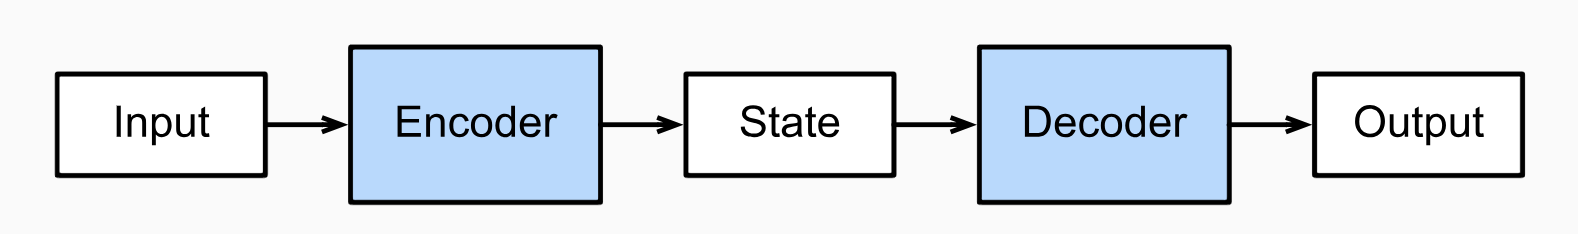
\includegraphics[width=0.65\linewidth]{fig/enc-dec.png}
    \caption{Encoder-Decoder Architecture}
\end{figure}

Encoder-decoder architectures can successfully be employed in sequence to sequence tasks with varying input and output sizes, such as machine translation, text summarization, and more. 

\textcolor{red}{[Dive Into Deep Learning]}

\subsection{Limitations of Recurrent Networks}
Recurrent neural networks \textcolor{red}{[Reference]}, long short-term memory \textcolor{red}{[Reference]}, gated recurrent \textcolor{red}{[Reference]}, and similar recurrent networks, have been firmly established well-performing approaches in sequence modeling and transduction problems such as language modeling, machine translation, and other NLP problems.

Recurrent models typically compute along the symbol positions of the input and output sequences. This means that they perform their computations sequentially. They learn a sequence of hidden states $h_t$ as a function of the previous hidden state $h_{t-1}$ and the input for position $t$. This sequential nature of processing limits parallelization within training examples, which becomes a problem with longer sequences as memory constraints limit batching across examples and training times increase. 

Moreover, these models can not quite capture the long-term dependencies and contexts of longer sequences. To mitigate these problems and improve model performance, a ground-breaking architecture called the Transformer Network was proposed in 2017 \textcolor{red}{[Transformer]}. The Transformer uses the following mechanisms in its architecture: \\[-20pt]
\begin{enumerate}
    \item Self-Attention \\[-20pt]
    \item Multi-Head Attention \\[-20pt]
    \item Positional Encoding \\[-20pt]
    \item Batch Norm \\[-20pt]
    \item Residual Connections \\[-20pt]
    \item Masked Multi-Head Attention \\[-20pt]
\end{enumerate}

We will first discuss some of these concepts briefly before providing the full Transformer architecture.

\subsection{Mechanisms in Transformer}
\subsubsection{Self-Attention}
To build up to the Transformer network, we need to first speak about its most fundamental component: \textbf{Self-Attention}.

Static Embeddings, as previously discussed, convert a token into a feature vector embedding that represents the token with a vector of numbers. Static embeddings, unfortunately, do not take the context of the token into account when creating the vector embedding. This is a limitation of the static embeddings learned using algorithms such as seq2vec.

To expand the idea of static embeddings to include contextualized information, self-attention is used to create contextualized embeddings that more adequately represent tokens in a sentence.

Self-attention inputs the input tokens ${X}$ and then uses three learnable weight matrices,

$$
\begin{align*}
&W^Q \in \mathbb{R}^{d_{\text {model }} \times d_k} \\ &W^K \in \mathbb{R}^{d_{\text {model }} \times d_k} \\&W^V \in \mathbb{R}^{d_{\text {model }} \times d_v}
\end{align*}
$$

to obtain the \textbf{query}, \textbf{key}, and \textbf{value} matrices,

$$
{
\begin{align*}
&Q = XW^Q  \\
&K = XW^K\\
&V = XW^V
\end{align*}
}
$$

which we will use to obtain $\green{A(Q, K, V)}$ contextualized embedding. The final equation for self-attention using these values is:

$$
\operatorname{Attention}(Q, K, V)=\operatorname{softmax}\left(\frac{Q K^T}{\sqrt{d_k}}\right) V$$

\subsubsection{Positional Encoding}
Another component of the Transformers is the \textbf{Positional Encoding}. Positional encodings are additional encodings that get added to the input encoding to inject positional information into self-attention. The reason for this is that self-attention on its own does not distinguish along positions and does not content itself with time-steps, therefore it would perform poorly with regards to learning positional patterns. The positional encoding provides the positional information needed for the model to achieve better spatial clarity and performance.

Many possible functions can be used for positional encoding, however, they must all have the following properties:

\begin{enumerate}
    \item \textbf{Not Ambiguous} - Have different values for different positions.
    
    \item \textbf{Deterministic} - It needs to be able to be calculated using the position values deterministically for the model to learn the position patterns.
    
    \item \textbf{Distance Encoded} - The encodings need to contain distance information; for instance, the encoding should allow the model to learn that position 1 is as far away as position 11 from position 6.
    
    \item \textbf{Work with sequences longer than encountered before} - It needs to work for sequences far longer than the sequences it is trained on.
\end{enumerate}

The positional encoding provided in the Transformer paper is the \textbf{sinusoidal positional encoding}.

The sinusoidal positional encoding assigns each position $p$ in the sequence a vector $P E(p)$ of the same dimension $d_{\text {model }}$ as the embedding vectors. This encoding is defined as:
$$
\begin{gathered}
P E(p, 2 i)=\sin \left(\frac{p}{10000^{2 i / d_{\text {model }}}}\right) \\
P E(p, 2 i+1)=\cos \left(\frac{p}{10000^{2 i / d_{\text {model }}}}\right)
\end{gathered}
$$

where $p$ is the position in the sequence, $i$ is the dimension index, and $d_{\text {model }}$ is the dimensionality of the encoding and token embeddings.

After obtaining the desired positional encodings (PEs), we have two options: either concatenate them with the input embeddings, which increases computational cost, or follow the approach suggested in the Transformer paper—adding the PEs directly to the input embeddings and allowing the model to learn their integration effectively.

$$
\tilde{\mathbf{x}}_t=\mathbf{x}_t+\mathbf{p}_t
$$

\subsubsection{Multi-Head Attenion}
As stated before, Transformers offer massive parallelization benefits due to their extensive use of attention. To facilitate this, multiple heads are performing attention at once. This is called the \textbf{Multi-Head Attention}. Here is its equation:
$$
\begin{aligned}
& \operatorname{MultiHead}(Q, K, V)=\operatorname{Concat}\left(\operatorname{head}_1, \ldots, \operatorname{ head}_{\mathrm{h}}\right) W^O \\
& \text { where } \operatorname { head}_{\mathrm{i}}=\operatorname{Attention}\left(Q W_i^Q, K W_i^K, V W_i^V\right)
\end{aligned}
$$


Where the projections are parameter matrices $W_i^Q \in \mathbb{R}^{d_{\text {model }} \times d_k}, W_i^K \in \mathbb{R}^{d_{\text {model }} \times d_k}, W_i^V \in \mathbb{R}^{d_{\text {model }} \times d_v}$ and $W^O \in \mathbb{R}^{h d_v \times d_{\text {model }}}$.

The process of multi-head attention can be observed in the following diagram.

\begin{figure}[h]
    \centering
    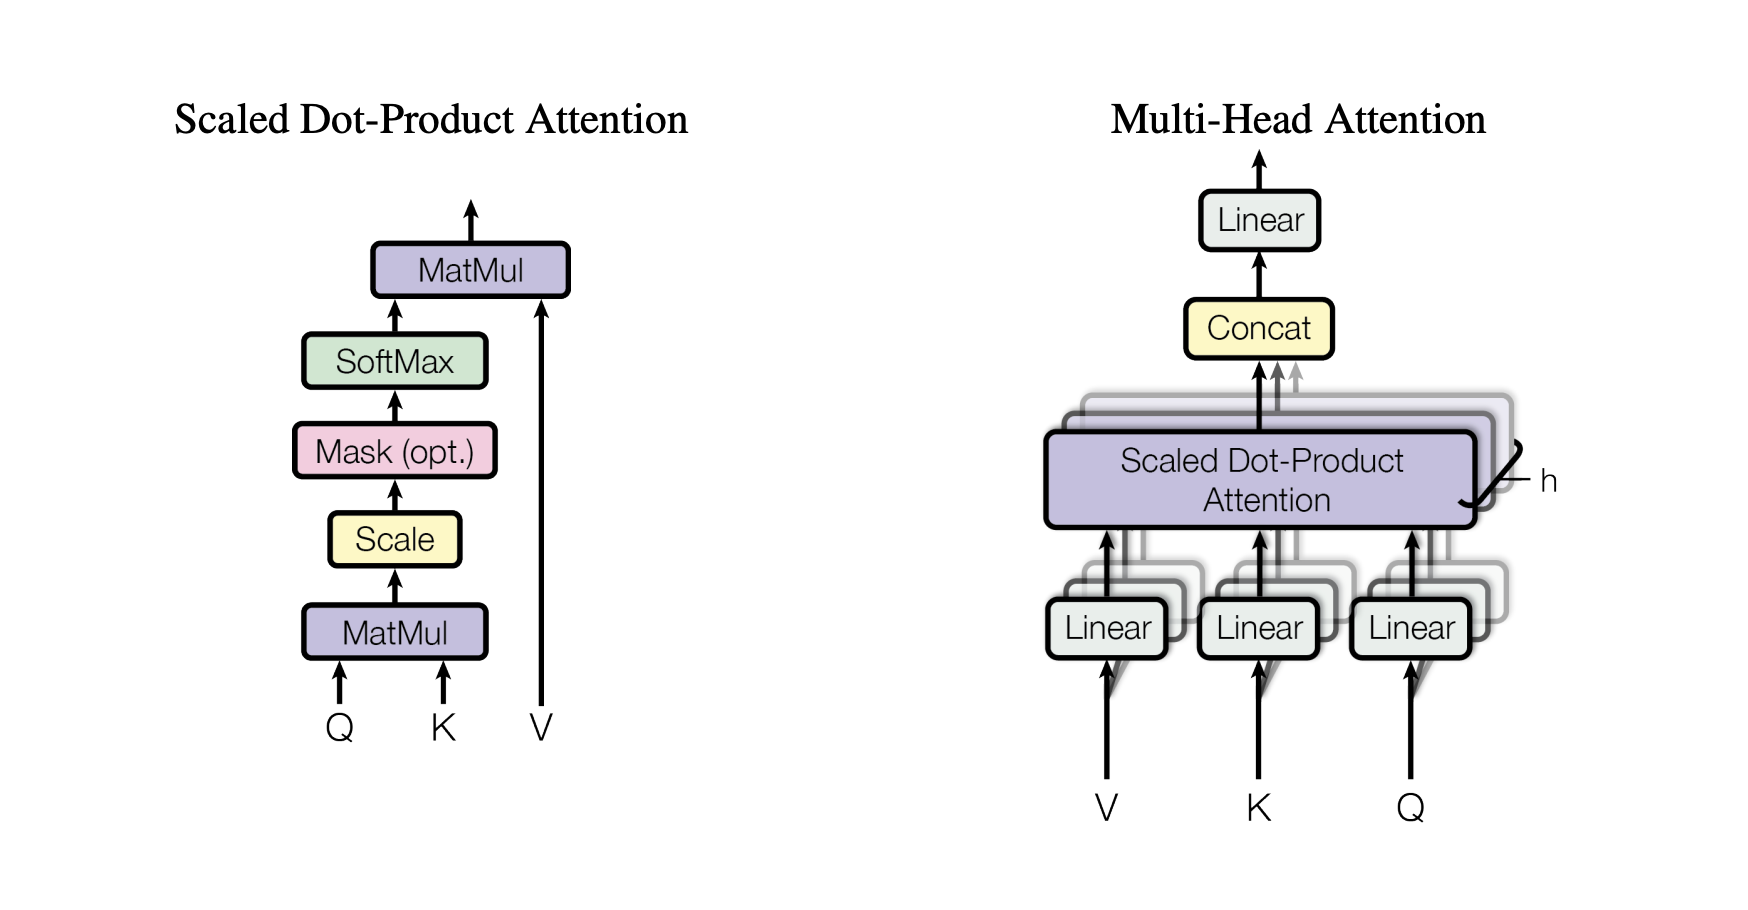
\includegraphics[width=0.9\linewidth]{fig/multi-head.png}
    \caption{Multi-Head Attention consists of several
attention layers running in parallel.}
    \label{fig:enter-label}
\end{figure}

In the original work, the authors chose $h=8$ attention heads. One more important point is that in multi-head attention, usually the $Q, K,$ and $V$ matrices are given to it as input, and there is no need to compute it, unlike in self-attention. However, if they are not provided in the input, they can be taken to be equal to $X$.

\subsection{Transformer Architecture (2017)}

Using the components discussed in the previous section, we can build the Transformer according to the encoder-decoder architecture as seen in figure \ref{fig:transformer}. In the original work, 6 encoder layers and 6 decoder layers were trained.

\begin{figure}[T]
    \centering
    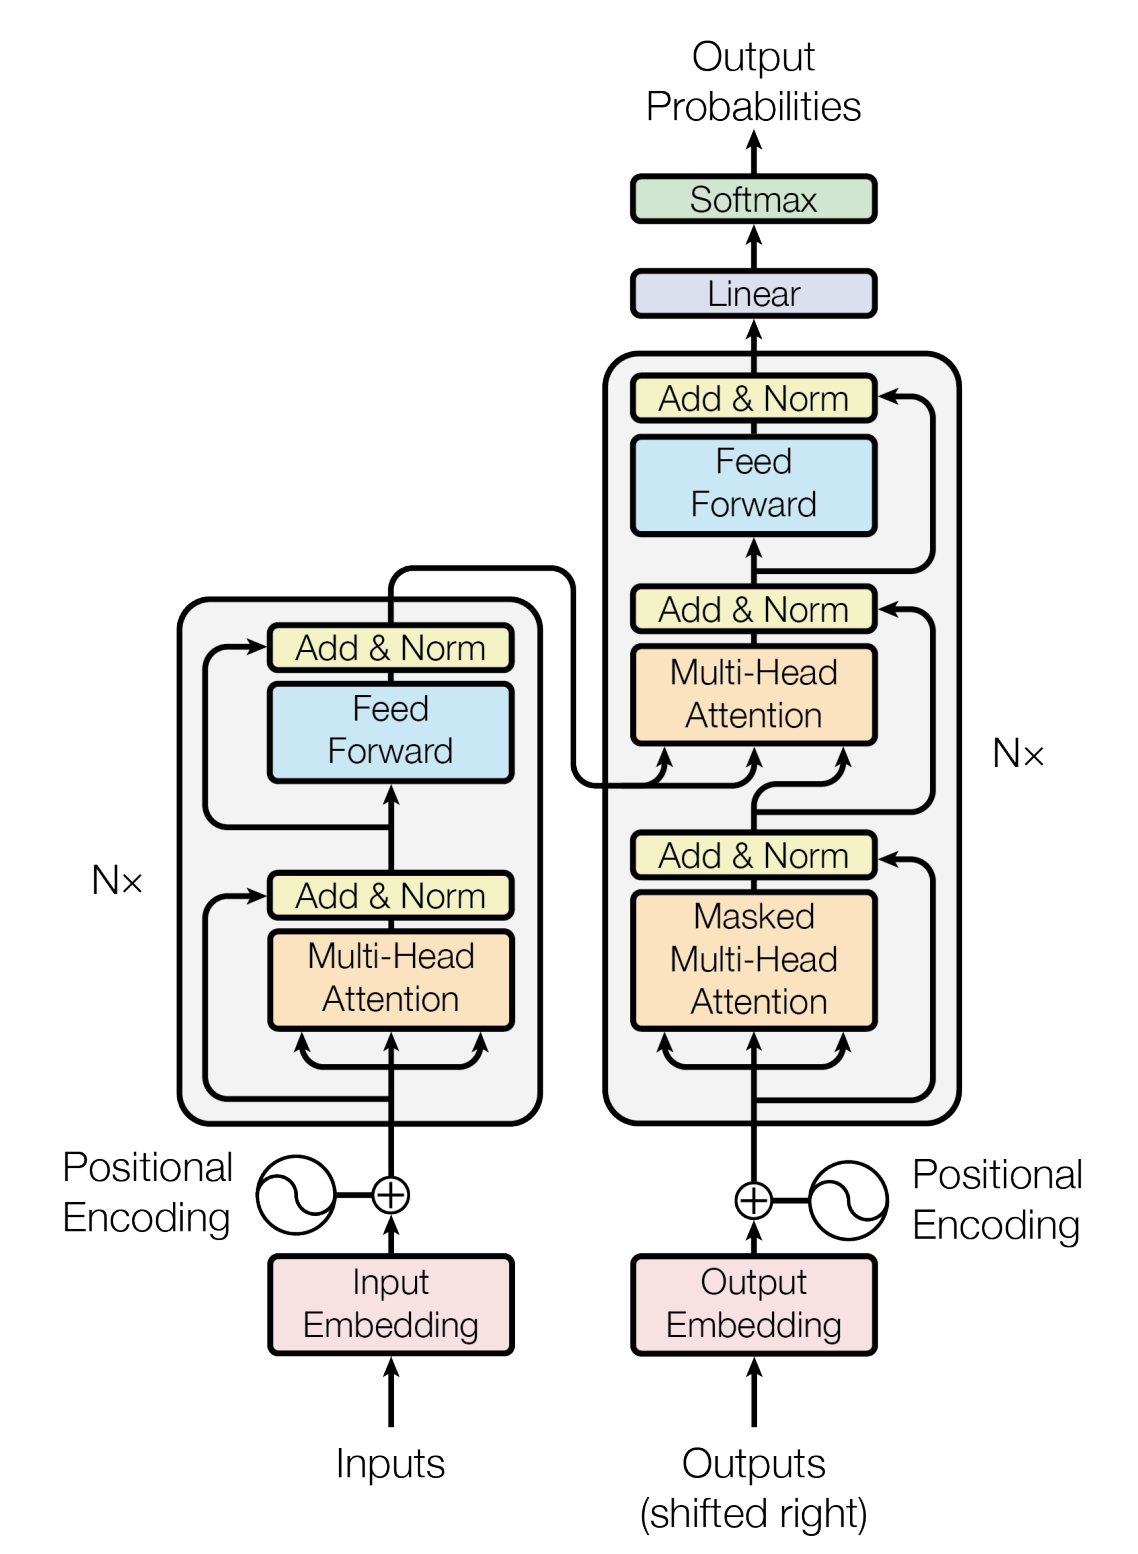
\includegraphics[width=0.65\linewidth]{fig/transfomer.png}
    \caption{Transformer Architecture}
    \label{fig:transformer}
\end{figure}

\subsection{Impact of Transformers}
Transformers were able to achieve state-of-the-art performance compared to the recurrent models. 
Ever since their introduction in 2017, Transformers have revolutionized the field of natural language processing and machine learning as a whole. 

Transformers became the foundation for a wave of groundbreaking models, such as BERT, GPT, and T5, which pushed the boundaries of tasks like translation, summarization, question answering, and text generation. The architecture also extended beyond NLP, impacting areas such as computer vision (e.g., Vision Transformers), time-series analysis, and even protein structure prediction (e.g., AlphaFold \textcolor{red}{[Reference]}). The introduction of pre-training and fine-tuning paradigms further solidified their impact, making domain adaptation efficient and accessible.

\section{Pre-Trained Models and Fine-Tuning}
Given the previous overview on Transformers, two fundamental concepts in NLP are pre-training and fine-tuning language models such as the Transformer. In most of the state-of-the-art language models seen today, these two concepts are used.

\subsection{Pre-Training}
Pre-training is the process of training a model on a large corpus of unlabeled data to learn a general-purpose understanding and representation of the language. This step typically uses self-supervised learning, where the model is trained to predict parts of the input based on the rest, without requiring manually labeled datasets.

Some tasks used for the self-supervised learning in pre-training include:

\begin{enumerate}
    \item \textbf{Masked Language Modeling (MLM):} In MLM, some input tokens are randomly masked, and the model is trained to predict these tokens based on their context. This task was used in the training of BERT\footnote{Bidirectional encoder representations from transformers}  model by Google in 2018 \textcolor{red}{[Reference]}.

    \item \textbf{Causal Language Modeling (CLM):} The model predicts the next token in a sequence given its previous tokens, operating in an autoregressive\footnote{Left-to-right} fashion. GPT\footnote{Generative pre-trained transformer} (2018) by OpenAI uses this approach, training models left-to-right.
\end{enumerate}

Pre-training allows for the learning of syntactic and semantic patterns of the language. These pre-trained models are then used as a foundation, significantly reducing the labeled data requirements for downstream tasks. In the larger pre-trained models improvement of performance can be achieve on diverse tasks.

\subsection{Fine-Tuning}
After pre-training is complete \textbf{Fine-tuning} is performed on a pre-trained model to purpose it for a specific task using labeled data. This step typically modifies the pre-trained weights slightly to optimize performance for the target task.

Transitioning from the pre-training and fine-tuning paradigms, we will explore BERT and GPT which are successful examples of using transformers as pre-trained models and then fine-tuning them to achieve great performance across NLP tasks.

\subsection{GPT (2018)}
GPT (Generative Pre-Trained Transformer) as the names suggest was a pre-trained model based on the decoder of the transformer introduced in 2018.  It introduced unsupervised pre-training followed by supervised fine-tuning. This model uses a unidirectional next word prediction task for training the model on multiple stacks of transformer decoders.

This pre-trained could then be fine-tuned by an output layer or component to specific NLP tasks such as question answering, translation, or text classification.

GPT was trained on the BooksCorpus dataset (a collection of about 11,000 unpublished books) and other publicly available datasets.

Here are some of the specifications of the GPT:

\begin{table}[H]
\centering
\renewcommand{\arraystretch}{1.5}
\setlength{\tabcolsep}{10pt}
\begin{tabular}{@{}lcc@{}}
\toprule
\textbf{Specification}          & \textbf{GPT (2018)}      \\ \midrule
Number of Transformer Layers    & 12                           \\
Number of Parameters            & 117M                         \\
Number of Multi-Head Attentions & 12                           \\ \bottomrule
\end{tabular}
\caption{Specifications of GPT }
\label{tab:gpt_specs}
\end{table}

The GPT achieved state-of-the-art performance in many tasks such as commonsense reasoning and question answering.


\subsection{BERT (2018)}

\begin{figure}[H]
    \centering
    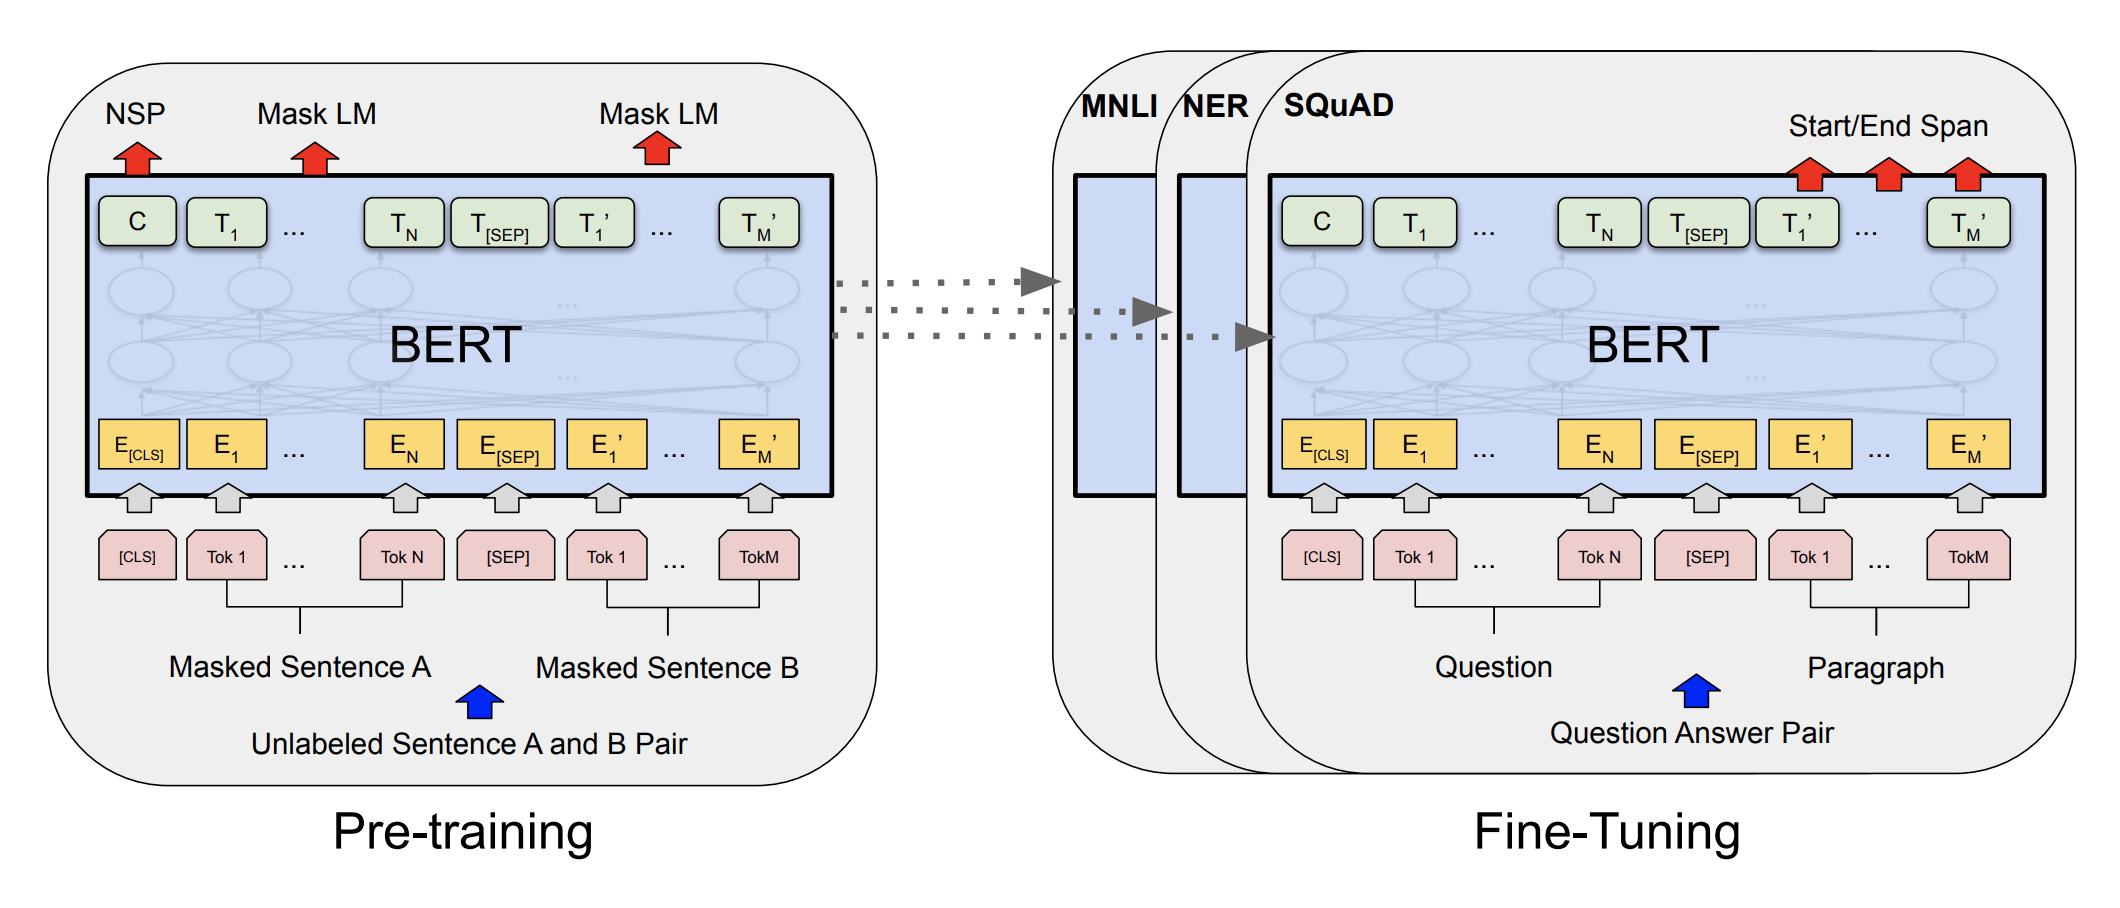
\includegraphics[width=0.9\linewidth]{fig/BERt.png}
    \caption{BERT Training}
    \label{fig:enter-label}
\end{figure}

\textbf{BERT (Bidirectional Encoder Representations from Transformers)} is a pre-trained language model introduced by Google in 2018. Unlike GPT, which is an autoregressive model generating text left-to-right, BERT uses bidirectional language representation by considering both left and right contexts. This bidirectional contextual understanding allows BERT to excel at tasks requiring a comprehensive understanding of the input text, such as classification and question answering.

BERT was pre-trained using only the encoder layer of transformer. One of the innovations of the BERT paper was the masked language model task which allows the model to learn bidirectionally by masking 15\% of the input tokens, either from left or right and asking the model to predict it.

Additionally, next sentence prediction task was also leveraged for model training. This task allows the model to understand the relationship between two sentences. The model is fed pairs of sentences and must predict whether the second sentence is the actual next sentence in the original text. This is particularly useful for tasks like question answering and natural language inference.


There were to versions of BERT released, BERT Base and BERT Large. Here are some specification relating to these two pre-trained models: \\

\begin{table}[H]
\centering
\renewcommand{\arraystretch}{1.5}
\setlength{\tabcolsep}{10pt}
\begin{tabular}{@{}lcc@{}}
\toprule
\textbf{Specification}           & \textbf{BERT-Base} & \textbf{BERT-Large} \\ \midrule
Number of Transformer Layers     & 12                 & 24                  \\
Number of Parameters             & 110M               & 340M                \\
Number of Multi-Head Attentions  & 12                 & 16                  \\ \bottomrule
\end{tabular}
\caption{Specifications of BERT-Base and BERT-Large}
\label{tab:bert_specs}
\end{table}


After pre-training, BERT can be fine-tuned for specific NLP tasks by adding a simple output layer. Fine-tuning adjusts the parameters of BERT slightly to adapt it to the specific task, such as text classification, question answering, named entity recognition, and more.

\section{GPT-2 and GPT-3}

\subsection{GPT 2 (2019)}
In 2019 GPT-2 was introduced. GPT-2 was step up from GPT in terms of its scale. It used a very similar architecture to GPT, however it was much larger which allowed it to have boosted performance across different tasks. It kept the transformer decoder-based self-supervised style of training a pre-trained model and supervised fine-tuning.

It was trained on a dataset of approximately 8 million web pages scraped from the internet (WebText) which was about 40 GB of data.

\subsection{GPT-3 (2020)}
GPT-3 was another state-of-the-art language model developed by OpenAI and released in 2020. It represented a significant advancement over its predecessor, GPT-2, in terms of scale, capabilities, and versatility. It kept the same architecture but yet again increased scale and improved learning methodology.

The model was pre-trained on a massive and diverse dataset of internet text which was about 570 GB large.

The following table shows the specifications of GPT 1 through GPT 3 compared against one another. \\

\begin{table}[H]
\centering
\renewcommand{\arraystretch}{1.5}
\setlength{\tabcolsep}{12pt}
\begin{tabular}{@{}lccc@{}}
\toprule
\textbf{Feature}       & \textbf{GPT-1 (2018)}     & \textbf{GPT-2 (2019)}       & \textbf{GPT-3 (2020)}       \\ \midrule
Layers                 & 12                 & 48                   & 96                   \\
Parameters             & 117M               & 1.5B                 & 175B                 \\
Hidden Size            & 768                & 1600                 & 12,288               \\
Attention Heads        & 12                 & 25                   & 96                   \\
Vocabulary Size        & 40,000             & 50,257               & 50,257               \\
Context Length         & 512                & 1024                 & 2048                 \\ \bottomrule
\end{tabular}
\caption{Specifications of GPT-1, GPT-2, and GPT-3}
\label{tab:gpt_specs}
\end{table}


\subsection{Zero-Shot and Few-Shot Learning}
\textbf{Zero-shot learning} is paradigm where a model generalizes to new tasks or classes without seeing any labeled examples for those tasks during training.

\textbf{Few-shot learning} on the other hand is an approach where an ML model learns to perform a task or classify new classes with only a few labeled examples per class. It leverages prior knowledge from large-scale pretraining or meta-learning to adapt quickly to data-scarce scenarios.

While few-shot learning has been explored conceptually and in limited applications before, the practical realization and broad applicability of few-shot learning in NLP truly started with OpenAI's GPT-3 in 2020. GPT-3 displayed the ability to perform a wide range of tasks by using few-shot prompts, stopping the need for task-specific fine-tuning and changing how language models are used in practice. GPT-3 was capable of this due to its massive size and long training which resulted in a pre-trained model that has learned language representations well enough to be able to perform few-shot learning adequately. In some tasks, few shot learning on GPT-3 performed similarly to models fine-tuned to perform that task. GPT-3 also showed capability of performing zero-shot learning as well.

As an example of few-shot prompts consider the following input to a pre-trained large language model (4-shot prompt):

\hrulefill

\texttt{\textcolor{blue}{Text:} (lawrence bounces) all over the stage, dancing, running, sweating, mopping his face and generally displaying the wacky talent that brought him fame in the first place.
\\
\textcolor{blue}{Sentiment:} positive}

\texttt{\textcolor{blue}{Text:} despite all evidence to the contrary, this clunker has somehow managed to pose as an actual feature movie, the kind that charges full admission and gets hyped on tv and purports to amuse small children and ostensible adults.\\
\textcolor{blue}{Sentiment:} negative
}

\texttt{\textcolor{blue}{Text:} for the first time in years, de niro digs deep emotionally, perhaps because he's been stirred by the powerful work of his co-stars.\\
\textcolor{blue}{Sentiment:} positive}

\texttt{\textcolor{blue}{Text:} i'll bet the video game is a lot more fun than the film. \\
\textcolor{blue}{Sentiment:}
}

\hrulefill

\section{Modern Large Language Models (2020 -- Present)}
\subsection{LLMs}
GPT-3 is an example of a \textbf{large language model}. It is considered ``large" due to its massive amount of parameters (about 175 billion).

To formulate what constitutes an LLM\footnote{Large language model}, we can state some properties LLMs generally have:
\begin{enumerate}
    \item \textbf{They have tens of billions of parameters}, e.g. 1.76 trillion parameters on OpenAI's GPT-4.
    \item \textbf{They are trained on a massive and diverse corpus of text}, e.g. Meta's LLaMA was trained on about 1.4 TBs of text.
    \item  \textbf{They are capable of generalization such as zero-shot and few-shot learning}.
    \item \textbf{They often support a large context window.}
    \item  \textbf{They require significant computational resources for training and inference}, e.g. Google's Gemini Ultra cost about 190 million dollars to train.
\end{enumerate}

Now, we will briefly mention some of the modern LLMs that have taken the world by storm. It will become apparent that most LLMs today are trained in the industry rather than in academia.

\subsection{OpenAI's GPT-3.5 (2022)}
GPT‑3.5 marked a turning point in making large language models broadly accessible. Originally used as the backbone for ChatGPT when it launched in late 2022, GPT‑3.5’s conversational fluency and general-purpose language understanding impressed millions of users who had never before interacted with AI at such scale. Its underlying architecture was an evolution of GPT‑3, the refinement in dialogue management and context awareness made it a favorite for applications ranging from customer support to creative writing. This model’s success helped fuel a wave of public enthusiasm and research investment in conversational AI technologies.

\subsection{OpenAI's GPT-4 (2023)}
Launched in March 2023, GPT‑4 took the capabilities of its predecessor to a new level by incorporating multimodal inputs and improved reasoning skills. It expanded context window and the ability to process both text and images. Its performance improvements on professional exams and coding tasks caused both scientific admiration and commercial hype. GPT‑4’s integration into products like ChatGPT Plus and Bing Chat underscored its market impact and solidified OpenAI’s leadership in generative AI research.

\subsection{Google's Gemini (2023)}
Google’s Gemini released in 2023 as a rival in the race for multimodal intelligence. Designed to handle text, images, and even video, Gemini drew significant attention for its extended context lengths—up to millions of tokens—and robust integration of diverse data types. Gemini’s launch signaled Google’s determination to lead in next‑generation AI systems and sparked widespread debate about the future interplay between AI multimodality and practical application. Although a very powerful model, the market was mostly dominated by OpenAI's models due to their better overall performance and quality.

\subsection{OpenAI's GPT-4o (2024)}
Introduced in May 2024, GPT‑4o (with “o” standing for “omni”) pushed the envelope further by unifying text, image, and audio processing in a single model. Its design emphasized cost‑efficiency and speed while delivering state‑of‑the‑art performance on multilingual and multimodal benchmarks. The model quickly gained hype as it let more natural, humanlike interactions. By significantly reducing the cost per token compared to earlier models, GPT‑4o demonstrated that high‑performance multimodal AI could be both powerful and economically viable.

\subsection{OpenAI's o1 (2024)}
Released in late 2024, OpenAI’s o1 model was a breakthrough in advancing AI reasoning. Unlike its prediction‑only predecessors, o1 was designed to “think” through complex queries using reinforcement learning techniques that allowed it to explore multiple solution paths before giving an answer. This model excelled at challenging tasks in mathematics, coding, and scientific problem solving.

\subsection{Deepseek R1 (2025)}
Deepseek R1, released in January 2025 by a Chinese AI startup, has been regarded as a disruptive force in the AI landscape. This model achieved performance levels comparable to OpenAI’s advanced o1 series while costing a fraction of the price. This achievement has been regarded as an “AI Sputnik moment.” More importantly Deep Seek R1 is an open-source model unlike its OpenAI counterparts. Its release has caused intense discussion about international competitiveness in AI research. By demonstrating that reasoning and natural language understanding can be achieved with less costly training, Deepseek R1 has pushed scientific boundaries and reshaped market expectations for future AI development.





\end{document}


%\documentclass{article}
%\usepackage{hyperref}

% \begin{document}

The rise of powerful modern LLMs such as GPT-4-o and Google Bard has led many to believe we have already achieved "machine consciousness". But is this true? If it's true, how would we know it? If it's not, how far are we from it?

\section*{Are Modern LLMs Conscious?}

Instead of a philosophical discussion about what "consciousness" even is, we ask a much simpler question: "Are modern LLMs capable of reasoning?" This question has its fair share of both concurring and opposing opinions among academics. Although most academics believe that LLMs are not yet capable of reasoning.

But if they are not reasoning, what are they doing? In \textit{Can Large Language Models Reason} (\href{https://aiguide.substack.com/p/can-large-language-models-reason}{source}), Mitchell answers this question:

\begin{quote}
"If it turns out that LLMs are not reasoning to solve the problems we give them, how else could they be solving them? Several researchers have shown that LLMs are substantially better at solving problems that involve terms or concepts that appear more frequently in their training data, leading to the hypothesis that LLMs do not perform robust abstract reasoning to solve problems but instead solve problems (at least in part) by identifying patterns in their training data that match, or are similar to, or are otherwise related to the text of the prompts they are given."
\end{quote}

This is not cognition; it's merely mechanical perception.

\begin{quote}
"Some GPT-based LLMs (pre-trained on a known corpus) were much better at arithmetic problems that involved numbers that appeared frequently in the pre-training corpus than those that appeared less frequently. These models appear to lack a general ability for arithmetic but instead rely on a kind of "memorization"—matching patterns of text they have seen in pre-training. As a stark example of this, Horace He, an undergraduate researcher at Cornell, posted on Twitter that on a dataset of programming challenges, GPT-3 solved 10 out of 10 problems that had been published before 2021 (GPT-3's pre-training cutoff date) and zero out of 10 problems that had been published after 2021. GPT-3's success on the pre-2021 challenges thus seems to be due to memorizing problems seen in its training data rather than reasoning about the problems from scratch."
\end{quote}

This is quite an indictment of GPT’s problem-solving capabilities. However, there is a vigorous debate about what exactly LLMs “understand" and how different it is from how humans understand. On the one hand, most academics hold (\href{https://www.science.org/doi/10.1126/science.adj5957}{source}) that models trained on language “will never approximate human intelligence, even if trained from now until the heat death of the universe.” Not all researchers agree, claiming that “the behavior of LLMs arises not from grasping the meaning of language but rather from learning complex patterns of statistical associations among words and phrases in training data and later performing ‘approximate retrieval’ of these patterns and applying them to new queries.” So they might not be capable of "human reasoning" but they can be called capable of using "machine reasoning".

\section*{Can machines achieve human reasoning and understanding?}

There are a multitude of challenges. First and foremost, how will we see these technologies understand our world? Second, when will we have the tools to know how they can?

OpenAI disclosed that GPT-4 scored very well on the Uniform Bar Exam, the Graduate Record Exam, and several high-school Advanced Placement tests, among other standardized exams to assess language understanding, coding ability, and other capabilities, but evidence of human-level intelligence in GPT-4 is sketchy.

Critics claim that data contamination was at play. People taking standardized tests answer questions they have not seen before, but a system like GPT-4 may have very well seen them in the training data. OpenAI claims to use a "Substring Match" technique to search training data and tags for similar but not exact matches. OpenAI’s method was criticized in one analysis as “superficial and sloppy.” The same critics noted that “for one of the coding benchmarks, GPT-4’s performance on problems published before 2021 was substantially better than on problems published after 2021—GPT-4’s training cutoff. This is a strong indication that the earlier problems were in GPT-4’s training data. There’s a reasonable possibility that OpenAI’s other benchmarks suffered similar contamination.”

Shortcut Learning - ML and deep learning can cause unpredictable errors when facing situations that differ from the training data. This is because such systems are susceptible to shortcut learning; statistical associations in the training data allow the model to produce correct answers for the wrong reasons. Machine learning, neural nets, and deep learning do not teach concepts; instead, they teach shortcuts to connect responses to the training set and apply statistical associations and probability assumptions to produce correct answers without cognition of the intended query. Another study showed that “an AI system that attained human-level performance on a benchmark for assessing reasoning abilities relied on the fact that the correct answers were (unintentionally) more likely statistically to contain certain keywords. For example, answer choices containing the word ‘not’ were more likely to be correct.”

So whenever we might think that LLMs have achieved a level where they are able to solve a unique problem, it might be that there was another very similar problem in their vast amount of database. Or it might be that they came to the correct answer due to wrong reasons.

Basically, the problem of how to appropriately benchmark the level of human intelligence is still an open problem. But the most widely known criteria for assessing human intelligence is the "Turing Test."

The Turing test, originally called the imitation game by Alan Turing in 1949, is a test of a machine's ability to exhibit intelligent behaviour equivalent to, or indistinguishable from, that of a human. Turing proposed that a human evaluator would judge natural language conversations between a human and a machine designed to generate human-like responses. The evaluator would be aware that one of the two partners in conversation was a machine, and all participants would be separated from one another. If the evaluator could not reliably tell the machine from the human, the machine would be said to have passed the test.

This still might not be able to assess whether machines are capable of human reasoning. But to some extent, this can attest that they have achieved some level of human understanding.


\section*{What the future holds—Bridging the gap between A.I and humans—}

So far until now, the improvement of LLMs is mainly attributed to drastically increasing the size of Language Models. But it is unlikely that more improvement can be achieved in this regard and some major changes in architecture are needed. This has led many to analyze the process of the human mind in hopes of some motivation. We will explore some of these ideas.

\subsection*{Multimodal Models}
Nowadays we have achieved good results in approximating human information processing in all five of the human senses. In the strive towards AGI, one might suggest that "why not make a robot who can understand physical information like humans and then let it learn like humans" and the academics' answer to that is "why not?". This is the main idea behind a trend in LLMs to integrate already existing models for computer vision, image processing, etc., into LLMs.

\subsection*{Multidirectional Models}
A major difference between neural networks and the human mind is the fact that signals in neural networks travel from only one side to another. But the case of the human mind is not so simple. Multidirectional models are a way to mimic that sort of behavior in artificial neural networks.

\subsection*{Hybrid Models}
There’s growing interest in creating hybrid AI models that combine the best of both worlds:
\begin{itemize}
    \item Neural networks (like LLMs) for pattern recognition and dealing with unstructured data.
    \item Symbolic reasoning systems for applying formal logic, rules, and consistent deductions.
\end{itemize}
These hybrid models could bridge the gap between the probabilistic reasoning of LLMs and the symbolic, rule-based reasoning that humans excel at. This approach could allow AI systems to handle a wider variety of tasks with greater accuracy, from understanding natural language to performing complex logical deductions in fields like mathematics, law, or scientific reasoning.

%\end{document}







% \addcontentsline{toc}{section}{Bibliography}
% \bibliographystyle{unsrt}
% \bibliography{Biby.bib}

\end{document}
